
\documentclass[preprint,1p, 10pt,authoryear]{elsarticle}

\usepackage{multicol}
\usepackage{graphicx}
\graphicspath{{./Graphic/}}
\usepackage{array}
\usepackage{amssymb} % various useful mathematical symbols
\usepackage{gensymb} % for `degree' sign
\usepackage{amsthm}  % extended theorem environments
\usepackage{lineno}   % for line numbers
\usepackage{amsmath} % for math operations
\usepackage{mathtools} % for math operations
\usepackage{tabularx} % for adjustable table width
\usepackage[hidelinks]{hyperref}  % for hyperlinks
\usepackage{amsmath}
\newtheorem{property}{Property}[section]
\usepackage{soul}
\usepackage{xcolor}
\usepackage{epsfig}
\usepackage{amssymb}  % various useful mathematical symbols
\usepackage{tabularx}
\usepackage{multirow} 
\usepackage{colortbl}
\usepackage{tablefootnote}
\usepackage{footnote}   
\usepackage{setspace}
\usepackage{rotating}
\usepackage{adjustbox}
\usepackage{blindtext}
\usepackage[printwatermark]{xwatermark}
\usepackage{xcolor}
\usepackage{graphicx}
\usepackage{lipsum}

\journal{Journal of Geophysical Research: Solid Earth}


\begin{document}


\begin{frontmatter}



\title{Modeling precursory laboratory seismicity using a wear-based rate- and state-dependent friction model}

 \author[1]{P. A. Selvadurai \corref{cor1}}
 \ead{paul.selvadurai@sed.ethz.ch}
\author[2]{P. Galvez}
\author[2]{P. M. Mai}
\author[3]{S. D. Glaser} 
\author[1]{S. Wiemer} 



\cortext[cor1]{Corresponding author, Post-Doctoral fellow}
\address[1]{Swiss Seismological Service, ETH Zurich, Zurich, Switzerland}
\address[2]{King Abdullah University of Science and Technology, Thuwal, Saudi Arabia}
\address[3]{Civil and Environmental Engineering, University of California, Berkeley, California, USA}

%\begin{keypoints}
%\item Rate and state friction (RSF) models were developed from roughness measurements of a friction experiment that displayed properties of wear
%\item Simulations showed that smooth sections nucleated events that ruptured and were arrested by local roughened sections representing barriers
%\item Source properties of the RSF ruptures were compared to independently measured kinematic estimates from a concerted study for the first time
%\end{keypoints}


\begin{abstract}
We develop a rate- and state-dependent friction (RSF) model using the quasi-dynamic earthquake rupture simulator QDYN to investigate a compendium of recent experiments performed on a fault analog. A fault was sheared until macroscopic stick-slip frictional failure occurred. Before the macro-failure small precursory seismicity nucleated from regions that also experienced aseismic slow slip. The RSF model aims at understanding spontaneous shear events on fault patches that supported slow aseismic slip and associated nucleation processes. A key ingredient for this observation is heterogeneity, defined in our model as local variation in frictional parameters from the roughness.  The surface was characterized \textit{a posteriori} and displayed clear evidence of wear in the form of a bimodal Gaussian distribution of surface height. This unique superposition of smooth and rough Gaussian surface heights was used to impose spatial heterogeneity in critical slip distance $D_{c}$, which was equivalent to variations in fracture energy $G^{'}$.  The model revealed that local seismicity nucleated on the ``smooth/polished'' sections, while the larger ``rough'' section hosted aseismic slip. As the level of heterogeneity between smooth and rough sections increased, the model transitioned from a predominantly stick-slip to creep-like behavior.  The simulations produced a dominant asperity, which appeared to control aspects of rupture nucleation: ($i$) weak heterogeneity caused the dominant asperity to rupture in a regular manner but could also `cascade-up'  and produce a fault-wide event, while ($ii$) strong heterogeneity led to constrained rupture of the dominant asperity with repeating behavior. Seismic source properties: average slip $\delta$, seismic moment $M_{0}$, stress drop $\Delta \tau$ and fracture energy $G^{'}$, were determined for each event and agreed with separate kinematic estimates made independently from the experimentally measured ground motions produced by elastodynamic stress waves. Our numerical calculations provide insight into seismicity produced from frictional heterogeneity associated with worn faults in the laboratory.

\end{abstract}
%\section*{Plain Language Summary}
%Recent seismic observations show that faults experience a range of slip patterns spanning many scales in both space and time. Understanding how slip accumulates on complex fault systems can lead to a better understanding of regions that are more prone and susceptible to large events.

%We developed a friction model that we used to study results from a scaled frictional fault in the laboratory. This fault also showed complex slip behavior. We notice that scaled versions of earthquakes occurred in larger regions that were also slipping more slowly. This behavior has also been observed in nature but we are not certain as to why exactly. We linked this behavior to a mathematical model that describes friction on faults. To add complexity, we used the experimental roughness measured along the interface, which might explain the complicated slip patterns. Using the roughness, we found that the model produced earthquakes patterns and general behaviors that matched many experimental measurements taken independently. We found that complexity formed by fault roughness can produce a wide range of slip behaviors that are also observed in natural systems at many scales. Understanding how roughness evolves over a fault's lifetime will be important for moving forward earthquake science.  


\begin{keyword}
Earthquake nucleation, foreshocks, laboratory experiments, rate and state friction, wear, fault mirrors, asperities, seismic source properties
\end{keyword}

\end{frontmatter}
\doublespacing
\linenumbers



\section{Introduction}
\label{int}
Seismologic observations have captured a growing diversity in slip behavior along natural faults. Observations, such as spatio-temporally variations in seismicity rates \citep{Tormann2014, Tormann2015, Gulia2016,Gulia2019}, the presence of repeaters in aseismically creeping fault sections \citep[e.g.][]{Nadeau1994, Nadeau1999, Shirzaei2013, Uchida2019}, variations of slow slip distribution over large scales inferred from geodetic measurement  \citep[e.g.][]{Brodsky2014, Ruiz2014, Socquet2017}, the earthquake potential on sections prone to large ruptures \citep{Buergmann2000,Buergmann2004}, the observed variability in spatio-temporal slip patterns during rapid rupture \citep[e.g.][]{Mai2002, Tinti2005, Dreger2007, Galvez2016, Mai2018} suggest that coupling of faults and the ability to resist frictional breakdown is heterogeneous. 

Heterogeneity in frictional properties is also necessary to explain the observation that, in certain cases, precursory seismicity has been detected in regions that also support the steady growth of a preslip region \citep{Kato2012, Kato2016, Obara2016, Ruiz2014, Bouchon2013,Buergmann2004}. Preslip is a slow accumulation of fault slip in a region that grows outwards to a critical size where it becomes unstable and the mainshock ensues \citep{Ohnaka1992,Ben-Zion2008}. This portion of the seismogenic cycle is known as the nucleation phase. This behavior has been identified from the onset of the mainshock's seismogram \citep{Iio1995, Ellsworth1995, Beroza1996}, whilst recent improvements in geodetic measurements help to lower the detectable threshold and identify the nucleation phase over long time scales (months to years) and length scales (kms) \citep[e.g.,][]{Roeloffs2006,Ruiz2014, Socquet2017}.  In certain cases, precursory seismicity in the form of foreshocks has been observed prior to the mainshock \citep[e.g.,][]{Dodge1995, Dodge1996, Bouchon2011}. While it is unclear if all mainshocks are preceded by foreshocks \citep{Brodsky2014, Mignan2014, Seif2018} they are currently only identificable in retrospective analysis. Due to their forecasting potential, foreshocks have become important phenomena to study.

The study of the spatio-temporal growth of a preslip region  and its transition from slow (quasi-static) to fast (dynamic) slip has been well documented in laboratory experiments \citep{Dieterich1978,Okubo1984, Ohnaka1999, Nielsen2010, Latour2013, Fukuyama2018, Zhuo2018, Ke2018, Buijze2020}. More recently, along with measuring the spatio-temporal evolution of a slow preslip region, acoustic emission sensors were deployed to detect localized, high-frequency and impulsive events that spontaneously emanate from sections of the fault that also hosted the preslip front \citep{Ma2002, McLaskey2013, Selvadurai2015,Passelegue2017, Zhuo2018a}.  Analysis of these localized events using seismological models found the moment released with respect to their geometry scaled with earthquakes in nature \citep{McLaskey2014, Selvadurai2019}. This similarity has sparked more interest in understanding the implications that laboratory foreshocks have on the growth and stability of the preslip region and the influence of foreshocks themselves on the size and timing of the larger mainshock \citep{McLaskey2019}.  A major question is when does a foreshocks `cascade-up' into the mainshock? Studies of the initial onset of seismic rupture using seismograms suggest that asperities exist at many spatial scales, and that the triggering of a cascading-style failure mechanism might stem from failure of a smaller section \citep{Okuda2018, Ide2019}. This type of hierarchical breakdown may indicate the existence of a hierarchical plate interface structure \citep{Ide2005, Aochi2014, Aochi2017}.  Foreshocks might be local failures of these asperities that do not fully `cascade-up' but do posses this runaway potential if conditions are favourable. 

Conditions that controls the occurrence of foreshocks (or other types of precursory seismicity) during the nucleation phase, even at laboratory scales, is not entirely clear. In previous laboratory foreshocks studies \citep{McLaskey2013, Selvadurai2015}, fault behavior was dictated by a dry and gouge-free fault environment.  In these cases, heterogeneity is believed to occur because of geometric interaction between two rough surfaces that give rise to contact asperities with locally high normal stresses.  The contact heterogeneity was confirmed by \citet{Selvadurai2017} with measurement of spatially variable normal stress determined from a pressure sensitive film placed along the rough-rough interface; this has also been widely investigated in the field of statistical contact mechanics \citep[e.g.][]{Greenwood1966,Johnson1985, Persson2006}. 

The relationship between contact heterogeneity and mechanisms explaining spontaneous occurrence of foreshocks in sections of accumulating slip were examined. \citet{Selvadurai2017} proposed that localized precursory events occurred on asperities that exhibit higher levels of normal stress, thus locally decreasing its critical nucleation length scale (defined later in Section \ref{Theory}). If the asperity was geometrically large enough with locally high normal stress, favorable conditions allowing for the spontaneous localization of foreshocks could occur in the preslip region. This hypothesis is also discussed by \citet{McLaskey2019}. Another mechanism proposed by \citet{McLaskey2013} was that the increased stressing rate around the local geometric interference between surfaces might contribute to higher shear stresses resulting in the dynamic failure of these contact asperities.  

But why do the foreshocks arrest? What type/level of frictional heterogeneity is necessary to arrest the rupture that should, on a homogeneous interface, continue to rupture over the entire frictional interface? From the study of dynamic rupture propagation, after spontaneous initiation of dynamic rupture, the slip front begins to expand in a crack-like manner, accelerating outwards to a critical velocity, whereby it may transition to a pulse-like dynamic rupture \citep{Heaton1990, Meier2016}. Experiments and numerical investigations into the causes of complex rapid rupture nucleation and arrest in the laboratory are highly dependent on the stress states on the fault ahead of the rupture \citep{Rubinstein2004, Rubinstein2006, Ben-David2010,Svetlizky2014,Fineberg2015, Maegawa2010, Tromborg2011, Kammer2012, Gabriel2012, Kammer2015} and appear to control even slower quasi-static ruptures \citep{Selvadurai2017a}. The study of why/how laboratory ruptures arrest in these studies are performed at larger scales than the high-frequency foreshocks measured with AE sensors. For this reason, it becomes difficult to investigate the interaction of the foreshock/nucleation region which requires, in the laboratory, a broadband temporal and spatial understanding of slip: from frequencies ranging from DC to $\sim$ 1.5 MHz and length scales ranging from tens of microns to meters. 

In this study, we aim to understand mechanisms for localized fast ruptures embedded within a slow rupture where asperities are formed from geometric mismatch of the two rough surfaces. We apply a numerical rate- and state-friction (RSF) model \citep{Dieterich1979,Ampuero2008, Rubin2005} to explain a compendium of laboratory data from a specific direct shear friction experiment performed on a fault analog. The observations follow recent publications the reader may consult for experimental details,

\begin{enumerate}
    \item \citet{Selvadurai2015} looked at the nucleation phase where a slow preslip front was observed prior to onset of system wide stick-slip instabilities. Within this preslip region, localized foreshocks were observed;
    \item \citet{Selvadurai2017} investigated characteristics of the roughness and quantitative analysis of the contact stresses on the asperities were documented;
    \item \citet{Selvadurai2019} estimated seismic source properties of the localized foreshocks events that occurred in the preslip nucleation region were quantified using kinematic source models.
\end{enumerate}


\subsection{Summarized Experiment}
\label{GeneralExp}
A schematic diagram of the direct shear friction apparatus is presented in Figure \ref{fig1}(a). We refer to this scale as the macrosopic scale for the discussion. Experiments consisted of loading a long slender PMMA slider (12.7 mm x 406 mm x 80 mm) onto a larger PMMA base plate (610 mm x 305 mm x 51 mm); the interacting faces of the PMMA slider block and base plate were first sandblasted. During an experiment, the fault was maintained under constant normal load $F_{n}$.  The top slider was driven at a constant macroscopic loading rate $V_{LP}$ and an in-line shear load cell was used to measure the bulk frictional resistance $F_{S}$ along the fault (see Figure \ref{fig1}(b)).   
  
\begin{figure}
 	\centering
 	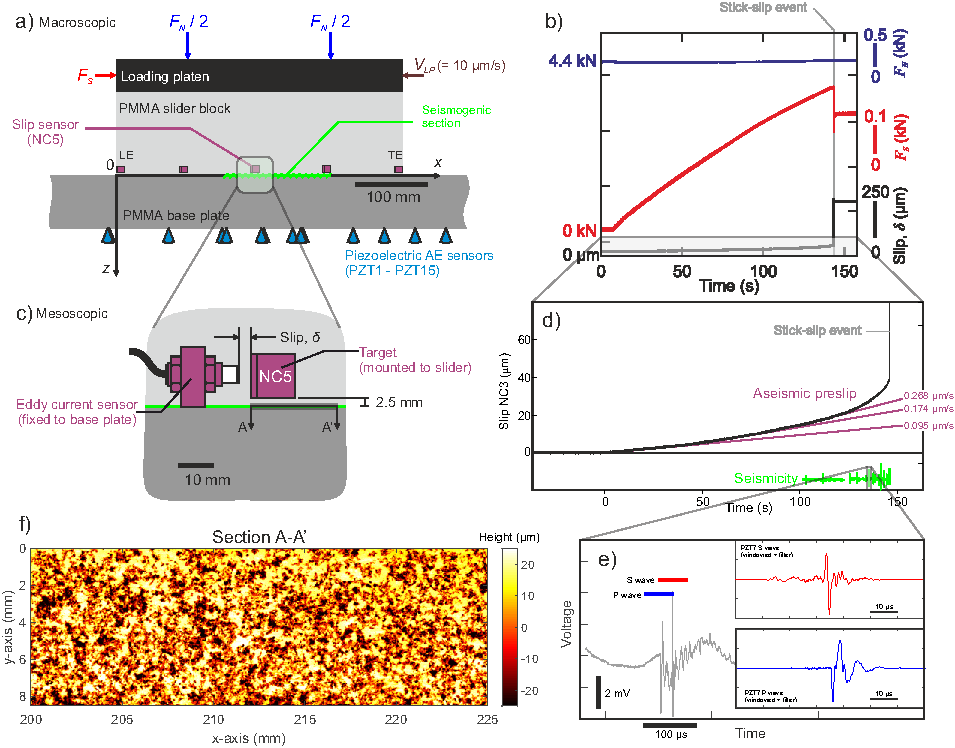
\includegraphics{FIG1_revised.pdf} 
 	\caption{ \textbf{(a)} Schematic details of the direct shear friction apparatus, depicting the general loading conditions and sensor placements are displayed. For more technical details please consult \citet{Selvadurai2015, Selvadurai2015a}. \textbf{(b)} Typical result demonstrating the bulk frictional evolution in terms of shear slip and shear force leading up to failure. \textbf{(c)} Schematic details of the non-contact eddy current sensor placement at the mesoscopic scale. \textbf{(d)} Detailed slip measurement during the experiment presented in (b).  Mesoscopic slow aseismic slip was observed prior to macroscopic stick-slip failure.  Lines of constant slip velocity are displayed for reference.  Seismicity (green) is represented schematically to document presence of local fast slip as the accelerated aseismic slip was observed. \textbf{(e)}  Example of precursory seismicity recorded using PZT7.  Seismicity showed clear P and S wave arrivals. More detailed source analysis has been performed by \citet{Selvadurai2019}. \textbf{(f)} Surface roughness measurement taken \textit{a posteriori} using the longer length scale optical profilometer (Nanovea P50).  The region on the fault associated with this scan is highlighted by the cross-section A-A’ in (c).}
 	\label{fig1}
 \end{figure}
In Figure \ref{fig1}(b) the slip evolution (black line) for the stick-slip event as measured by the non-contact eddy current sensor (NC5).  Figure \ref{fig1}(c) depicts a schematic representation of the eddy current sensor (mounted on the base plate) and the wing target attached to the slider block $\sim$ 2.5 mm on above the interface.  The inductive eddy current sensors measured slip $\delta$ in the $x$-direction. We refer to this scale as the mesosopic scale for the discussion.
 
During a stick-slip cycle, the slow and smooth accumulation of aseismic slip is detailed in Figure \ref{fig1}(d); lines of constant slip rate (magenta) are superimposed over the slip evolution curve.  The fault displayed an acceleration of aseismic slip leading to the stick-slip event. This type of observation is fairly common in laboratory friction experiments. However, we also observed pronounced impulsive events, detected using an array of absolutely calibrated piezoelectric transducers (PZT) that measure high-frequency vibrations (100kHz to 1500 kHz) produced by stress waves. Seismicity is represented schematically (green) since the time scales between the slow slip and this impulsive source were $\sim$ 6 orders of magnitude different.  Figure \ref{fig1}(e) depicts isolated P and S waves from a typical impulsive source measured by PZT7  \citep{Selvadurai2019}.
 
Our friction model requires spatial heterogeneity to explain the observations of synchronous and concomitant slow (Figure \ref{fig1}(d)) and fast rupture (Figure \ref{fig1}(e)). In our RSF model we base spatial heterogeneity  on the experimental \textit{a posteriori} measurement of surface roughness. Figure \ref{fig1}(f) presents the optical scan of surface roughness on the top slider block surface through the cross-section A-A' in Figure \ref{fig1}(c). The scan was taken below the non-contact sensor NC5.

\subsection{Surface Roughness Analysis}
\label{SRA}

Roughness has been proposed as a controlling feature linked to variability in frictional behavior on faults \citep{Scholz1986,Scholz2002}. Studies of the roughness of large exposed outcrops have been used to develop models describing the heterogeneity in stress and strength on active faults \citep[e.g.,][]{Schmittbuhl2006}. Large sections of exposed fault exhibit Gaussian distribution in roughness \citep[e.g.,][]{Renard2006} and can be characterized using the PSD of the surface height in terms of the fractal Hurst exponent \citep{Power1991, Schmittbuhl1995, Candela2009}. Increasingly smoothed faults have been found to be characterized by higher values of the Hurst exponent \citep{Brodsky2011, Siman-Tov2013, Kirkpatrick2014, Candela2016, Brodsky2016}.

We briefly describe methods used to quantify surface roughness in the fields of contact mechanics, tribology and geophysics that we will then use to characterize the interface presented in Figure \ref{fig1}(f). We measure average roughness as the root mean square:
\begin{equation}
h_{rms} = \sqrt{\left(\frac{1}{N} \right) \sum^{N}_{i=1} h_{i}^{2}} ,
\label{eq99}
\end{equation}
\noindent where $N$ is the total number of measurement points and $h_{i}$ is the individual surface height. To estimate statistical properties of surface heights we also employ the probability density functions (PDFs) of the surface height $h$ defined by a Gaussian distribution, given as follows:
\begin{equation}
\phi(h) = \left( 2\pi \sigma^{*} \right) exp\left[ \frac{\left(h - \mu^{*}\right)^{2}} { 2\sigma^{*2}}  \right],
\label{eq1}
\end{equation} 
\noindent where $\mu^{*}$ is the arithmetic mean and $\sigma^{*}$ is the standard deviation. Building on equation \eqref{eq1} the PDF for a bimodal Gaussian mixture model is given by 
\begin{equation}
\Phi(h) = p\cdot \phi_{1}(h)+\left(1-p\right)\cdot \phi_{2}(h),
\label{eq2}
\end{equation}
\noindent where $p$ is the mixture ratio between the two Gaussian distribution functions $\phi_{1}$ and $\phi_{2}$, each with their individual means and standard deviations. When fitting \eqref{eq1} and \eqref{eq2} to the experimental measurements we employ a maximum likelihood estimation (MLE) of the means, standard deviations and mixture ratio. 

Finally, we estimate surface properties using power spectral density (PSD), i.e.  the square of the modulus of the normalized Fourier transform, of a self-affine surface profile following 
\begin{equation}
P(k) \propto k^{-(1+2H)},
\label{eq999}
\end{equation}
\noindent where $k$ is the wavenumber and $H$ is the self-affine scaling exponent or Hurst exponent \citep{Power1991, Schmittbuhl1995, Mai2002, Candela2009}. By plotting equation \eqref{eq999} we can estimate $H$ using linear regression of log-log slope of the relationship between the PSD and wavenumber $\beta =-(1+2H)$.  

\subsection{Evidence of fault wear}
\label{SurfaceWear}
The facilities and measurement techniques are discussed in detail by \citet{Selvadurai2017}.  Figure \ref{fig2}(a) displays estimates of surface roughness using the root mean square (16.7 $\mu$m using equation \eqref{eq99}), Gaussian (equation \eqref{eq1}) and bimodal Gaussian (equation \eqref{eq2}) distributions for the surface presented in Figure \ref{fig1}(f). The values of the means ($\mu^{*}$), standard deviations ($\sigma^{*}$) and mixture ratio ($p$), are given for the modal (magenta) and bimodal (cyan), models with units of $\mu$m. The shape of the distribution is most adequately characterized by the bimodal Gaussian distribution.  Evolution of roughness from Gaussian to bimodal Gaussian can be quantified using the polish-rate decay (wear decay or \textit{Borucki} wear) function \citep{Adachi2000, Borucki2002, Borucki2004, Ciavarella2016,He2017,Hu2019}. This type of distribution has been well-documented in the field of tribology and is used to characterize wear of the interface. As the surface wears from a Gaussian to bimodal Gaussian it reaches a steady state roughness.  This worn characteristic was likely due to the lapping procedure described in \citet{Selvadurai2015} in which  $\sim$ 36.1 mm slip was used to precondition the fault surface before any experiments were reported. From the metrics, we see that wear has produced a smoother surface (i.e.  the `tail' in the PDF), and this polished surface exists within an encompassing rougher surface.     

\begin{figure}
	\centering
	\includegraphics{FIG2_revised.pdf} 
	\caption{\textbf{(a)} Surface height probability density function for the surface  in Figure \ref{fig1}(f). Values of three surface roughness models are established for the root mean square (black), Gaussian (magenta) and bimodal Gaussian (cyan) -- the values are given in $\mu$m. \textbf{(b)} Estimate of the Hurst exponent from the same surface are estimated from the power spectral density (PSD) described by equation \eqref{eq999} along the all transects in the $x-$direction (gray lines). The mean PSD for this surface is displayed in black and the Hurst exponent $H$ = 0.43 (red line) was estimated. \textbf{(c)} Image of the worn PMMA fault surface from \citep{Selvadurai2015b} reveals dark, smooth spots that are indicative of worn sections of the PMMA slider block. \textbf{(d)} Post-processing highlights the darker smooth sections. The inset image displays the spatial complexity of the smooth region. \textbf{(e)} Exposed outcrop with a mirror surface on a fault located along the Dead Sea Transform (image adapted from \citet{Goldberg2016}).  \textbf{(f)} Exposed outcrop with striated, glossy surface of the Corona Heights Fault (USA) (adapted from \citet{Verberne2019}).}
	\label{fig2}
\end{figure}
Figure \ref{fig2}(b) marks the Hurst exponent estimated using the power spectral density from the surface roughness transects in the $x-$direction. The average PSD was used to estimate a Hurst exponent $H$ = 0.43 between the wavenumbers of 1 mm $^{-1}$  $<k<$  50 mm $^{-1}$ from equation \eqref{eq999}. We note that any deviations of the values presented here from those in \citet{Selvadurai2017} are due to the more accurate cropping of the measurement region presented in Figure \ref{fig1}(f). 

Figure \ref{fig2}(c) reveals a raw photograph of the surface of the seismogenic section of the fault \citep{Selvadurai2017}, revealing polished spots with a ``mirror-like'' finish that was responsible for the tail in the PDF of the surface roughness. From \citet{Selvadurai2017}, the polished surface `mirrors' were 188 times smoother than the overall RMS roughness for the full region ($h_{RMS}$ = 16. 7 $\mu$m). Figure \ref{fig2}(d) highlights the darker regions by converting the raw image from RGB to light intensity between the range of 0 $< I <$ 0.35 \citep{Gonzalez2009}. The inset image displays the complexity associated within the polished section.

The presence of fault-mirrors (FM) observed on natural outcrops have sparked interest from the geophysical community \citep{Fondriest2013,Kirkpatrick2013, Siman-Tov2013}.  Laboratory experiments have been crucial in understanding the mechanism surrounding the formation of FMs and the debate of whether the presence of a fault mirror can be used as an indicator of seismic slip \citep{Fondriest2013,Siman-Tov2013,Pozzi2018}, but they have also been reproduced during slow slip \citep{Tisato2012,Siman-Tov2015}, in high-temperature environments \citep{Pluymakers2017} and observed along glacial boundaries \citep{Siman-Tov2017}. Figures \ref{fig2}(e) and (f) show fault mirrors on the Dead Sea Transform and the Corona Heights Fault (USA), respectively, that formed at different scales.  \citet{Goldberg2016} believe that these FMs can potentially promote seismicity and are also more prevalent and can occur at lower slip-rates than previously though \citep{Verberne2019}.  While there are differences between the mechanisms controlling how surfaces polish and FMs develop on rock-rock interfaces in hydro-thermal environments and controlling their development on a plastic PMMA surface \citep{Bouissou1998}, we are  more interested in how the initial conditions of a ``smoother surface embedded in a rougher fault'' affect the frictional behavior using a RSF model. 

\section{Rate- and state-dependent (RSF) friction model}
\subsection{Theory}
\label{Theory}
The RSF constitutive friction law is phenomenological and derived from laboratory experiments \citep{Dieterich1979, Ruina1983}.  The model describes the behavior of a fault's resistance to sliding in terms of shear stress $\tau$ as a function of slip rate $V$ and state variable $\theta$. This is given as:

\begin{equation}
\label{eq5}
\tau \left( V,\theta \right) = \sigma_{n} \left[\mu + a \ln\frac{V}{V^{*}} + b \ln\frac{V^{*}\theta}{D_{c}}\right],
\end{equation}   
\noindent where $\sigma_{n}$ is the normal stress, $\mu$ is the reference steady-state friction coefficient at an arbitrary reference slip rate $V^{*}$, $D_{c}$ is the characteristic slip distance and $a$ and $b$ are constitutive parameters describing the direct and evolution effects, respectively.  We adopt the state parameter in the form of the so-called "slip law" because of to its ability to model recent laboratory studies \citep{Bhattacharya2015, Kaneko2011, Kaneko2016}:

\begin{equation}
\label{eq6}
\dot{\theta} = - \frac{V\theta}{D_{c}}\ln\frac{V\theta}{D_{c}},
\end{equation}   

\noindent where friction at steady state ($\dot{\theta} $ = 0) is given as

\begin{equation}
\label{eq7}
\tau_{ss} \left( V \right) = \sigma_{n} \left[\mu + \left(a - b \right)\ln\frac{V}{V^{*}}\right].
\end{equation}   

\noindent From equation \eqref{eq7} we see that constitutive parameters $\left(a - b \right)$ play an influential role in how the interface behaves at steady-state.  For $\left(a - b \right) < 0$, $\tau_{ss}$ will decrease as slip rate $V$ increases.  A fault with these characteristics is known as velocity-weakening (VW) and is prone to spontaneous instability if the fault stiffness is below a critical stiffness. Stiffness of the VW spring-slider system was investigated by \citet{Ranjith1999} who found the critical stiffness to be:

\begin{equation}
\label{eq9}
k_{cr}=\frac{\sigma_{n} \left( b-a \right)}{D_{c}}.
\end{equation}   

\noindent  This implies that quasi-static steady-state slip is stable ($V \rightarrow V^{*}$) or unstable ($V \rightarrow \infty$) if the spring stiffness is greater than or less than the critical value $k_{cr}$, respectively. Fault stiffness is inversely proportional to the minimum half-length of a nucleation zone capable of instability:

\begin{equation}
\label{eq8}
L_{c} = \eta \frac{G^{*} D_{c}}{ \sigma_{n} \left( b-a\right)},
\end{equation}   

\noindent where $\eta = (7\sqrt{2})/(3\pi)$ \citep{Dieterich1992} for a square patch, the corrected shear modulus $G^{*} (= G/(1-\nu))$ was employed due to the Mode II plane strain conditions and $\nu$ is the Poisson's ratio. 

The equation of motion controlling slip on a planar fault is given by:

\begin{equation}
\label{eq8a}
\tau_{el}\left( \mathbf{x} \right) - \tau\left( \mathbf{x} \right) = \frac{G^{*}}{2 V_{S}} V(\mathbf{x}),
\end{equation}  

\noindent where $\tau_{el}$ is the elastostatic shear stress due to the loading boundary condition \citep{Horowitz1989}. The inertial term on the right hand side represents the radiation damping term for S waves produced along the fault at point $\mathbf{x}$, which expands at speeds closer to the shear wave speed $V_{S}$ of the material \citep{Rice1993}. 

Quasi-static interactions between fault elements are calculated using the boundary element method (BEM) and all calculations reported in this study were solved using a Quasi-DYNamic earthquake simulator \citep{Luo2017}. QDYN is a boundary element software designed to simulate earthquake cycles (seismic and aseismic slip on tectonic faults) under the quasi-dynamic approximation (quasi-static elasticity combined with radiation damping) on faults governed by RSF and embedded in elastic media.  Solution convergence and mesh discretization of the heterogeneous models described later is given in Supplemental Methods S1.

\citet{Dieterich1992} showed that RSF combined with elasticity leads to the common length scale

\begin{equation}
\label{eq8b}
L_{b} \equiv \frac{G^{*}D_{c}}{\sigma b}.
\end{equation}  

\noindent This characteristic dimension was later theoretically confirmed by \citet{Rubin2005} and controls aspects of earthquake nucleation and the transition from aseismic to seismic behaviour. We define this transition threshold to be:

\begin{equation}
\label{eq8c}
V_{dyn} = \frac{2 a V_{s}}{G^{*}},
\end{equation}  

\noindent which represents the transition point where the inertial term in equation \eqref{eq8a} becomes significant. 

\subsection{Recent advances in RSF modeling from the laboratory}
\label{advances RSF}
Experiments performed by \citet{Nielsen2010} and \citet{Latour2013} have benefited from increasing the fault's compliance using analog materials (glassy polymers) in frictional tests. In these experiments, improved spatio-temporal measurement of slip was achieved by using high speed digital cameras. Increased refinement in both spatial and temporal measurements clearly showed the so-called ``preslip'' or nucleation zone.  This nucleation region was predicted in RS models \citep{Dieterich1992, Rubin2005, Ampuero2008} but was difficult to show with high spatial resolution before novel sensing techniques.

Modeling efforts by \citet{Kaneko2011} and \citet{Kaneko2016} show that frictional behavior of the `plastic-on-plastic' sliding experiments can be explained using RS friction models. These models are informative and promote the idea of a `smooth transition' of frictional sliding over the macroscopic length scale of the experimental fault. It explains both the spatial and temporal evolution of observed nucleation features of those laboratory ruptures. While these studies have demonstrated that RSF are able to explain complex transients, neither addresses the role of fault roughness; they assume this is embedded implicitly in the phenomenological nature of the RSF parameters.

Roughness has been established to affect dynamic rupture propagation \citep[e.g.][]{Dunham2011, Fang2013}, nucleation physics \citep[e.g.][]{Tal2018} and the presence of aseismic transients \citep{Ozawa2019}. In these studies the fault is considered to be perfectly mated and roughness is described using the Hurst exponent. As the level of fault matedness in the modeled experiments was unclear at any time, we chose to use a \textit{cutting plane method} that discretizes frictional properties between the two surfaces (smooth and rough) defined in the bimodal Gaussian model.

\subsection{Cutting plane method}
The \textit{cutting plane method} splits the roughness into two separate sections: smooth and rough. Using this method we assign binary sets of frictional parameters to both the smooth and rough regions of the roughness profile. A `cutting plane' was defined to be exactly between the two means of the bimodal distributions that was formed due to wear. In this study, we build a simple 1-D model and arbitrarily choose the transect of the rough surface at $y$ = 2 mm. Figure \ref{fig3}(a) displays the roughness along $x$ at $y$= 2 mm (black line). In Figure 3(a), (b) and (c) the cutting plane (red) was defined as $h_{cut} = \left(\mu^{*}_{1}+\mu^{*}_{2} \right)/2$ = 12.54 $\mu$m using the bimodal Gaussian parameters calculated for surface heights along transect at $y = $ 2mm. Figure \ref{fig3}(b) depicts the probability distribution of the surface heights from the sample transect and the cutting plane in red. We assume that the ``smooth'' surface is the``upper'' one (above the cutting plane) that is characterized more effectively by the Gaussian distribution with lower standard deviation ($\sigma^{*}$), whereas the ``rough'' surface was below the cutting plane and had a larger standard deviation.

\begin{figure}[ht]
	\centering
	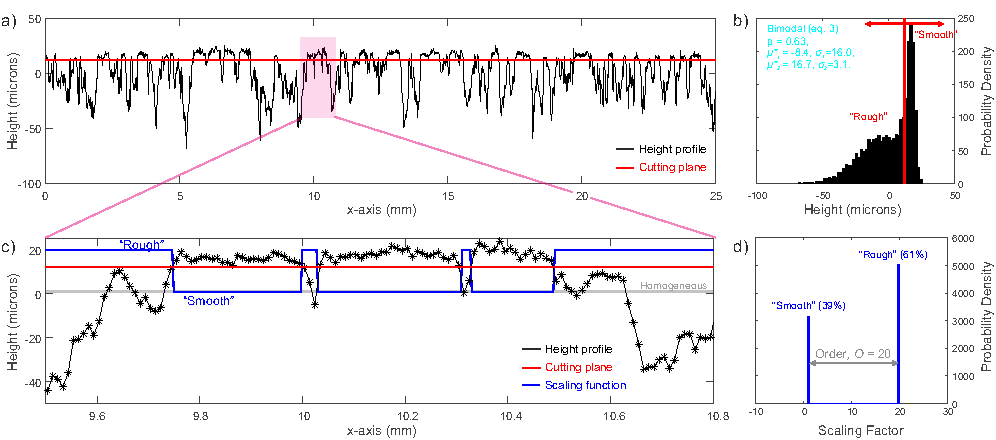
\includegraphics{FIG3_revised.pdf} 
	\caption{ \textbf{(a)} 1-D roughness profile (black) taken from the transect at $y$ = 2 mm in Figure \ref{fig1}(f).  The cutting plane $h_{cut}$ = 12.54 $\mu$m is used to separate the bimodal distribution into smooth and rough surfaces. \textbf{(b)} PDF of the height profile in (a) with the cutting plane (red vertical line). \textbf{(c)} Small section of the height distribution showing the roughness profile (black line), the cutting plane (red line) and the scaling function (blue line). \textbf{(d)} PDF of the scaling function $\mathrm{SF}(x)$ with an order of heterogeneity $O$ = 20.}
	\label{fig3}
\end{figure}

A scaling function ($\mathrm{SF}$) is used to partition the smooth and rough sections of the fault. Figure \ref{fig3}(c) marks a detailed view of the roughness (black), the cutting plane (red) and the scaling function (blue). When roughness was above the cutting plane the scaling function ($\mathrm{SF}$) was unity. All heights below the cutting plane were prescribed as scaled values. This allowed us to control the magnitude, or `order', of heterogeneity. For this example, the order was $O$ = 20. The  $\mathrm{SF}$ produced heterogeneity in two ways: (\textit{i}) spatial variations were controlled by the location where the roughness profile crossed the cutting plane, and ($ii$) the level (order) of heterogeneity -- the peak-to-peak range of SF -- was chosen by the modeler. The order of the $\mathrm{SF}(x)$ is clear seen in the PDF in Figure \ref{fig3}(d).

We approach the modeling in a non-traditional manner and imposed heterogeneity primarily through the frictional critical slip-weakening variable $D_{c}(x)$. Spatial fluctuations in fault roughness -- smoother and or rougher sections -- assumed properties based on arguments in past laboratory observations \citep{Marone1994}. Smooth sections were prescribed lower $D_{c,low}$, whereas rougher sections have a higher level of $D_{c, high}$. Spatial fluctuations in critical slip distance was given the lower value multiplied by the scaling function $D_{c}(x) = D_{c,low}\cdot$SF(x). The magnitude $D_{c}$ in the rough sections depended on the order $O$ of the scaling function. For example, for order $O$=20, the larger critical slip value was $D_{c, high} = \textrm{max}[D_{c}(x)] =$ 25 nm$\cdot$ 20 = 500 nm = 0.5 $\mu$m. This assumption also follows micro-mechanical simulations governing friction on dry, gouge-free interfaces \citep{Yoshioka1996,Yoshioka1997}. 

\subsection{Frictional parameter space}
\label{ParameterSpace}
Although we chose parameters based on our previous studies we also incorporated assumptions from the literature. The goal of our modelling is to identify conditions that produce local seismicity -- a critical experimental observation obtained from the PZT sensors. Figure \ref{fig4} demonstrates how the critical nucleation length $L_{c}$ (equation \eqref{eq8}) varies with $D_{c}$ and the normal stress $\sigma_{n}$.  Based on experiments performed by \citet{Berthoude1999} for PMMA, we set $a/b$ = 0.65 and $b$ = 0.0144. For reference, curves representing constant critical nucleation length are marked in red for $L_{c}$ = 25 mm and 0.9 mm.   

\begin{figure}
	\centering
	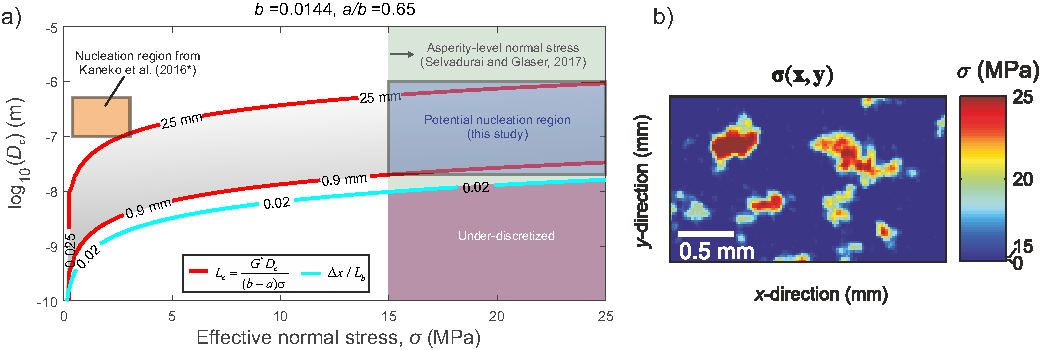
\includegraphics[scale = 0.95]{FIG4.pdf} 
	\caption{\textbf{(a) }Initial estimates of the nucleation parameter space ($L_{c}$) based on measurements of local normal stress \citep{Selvadurai2017}, minimum mesh discretization ($\Delta x /L_{b}$) and maximum critical nucleation size $L_{c} = 0.025$ m. The gray region represents possible nucleation sizes for the mesoscopic length scale.  The orange region represents the ranges of $D_{c}$ and normal stress $\sigma_{n}$ that nucleated full fault rupture in \citet[][, *$a/b$ = 0.6944]{Kaneko2016}. \textbf{(b) }Example of asperity-level normal stress field measured using an experimental pressure sensitive film \citep[adapted from ][]{Selvadurai2017} \citet{Selvadurai2017}.}
	\label{fig4}
\end{figure}

To further constrain our models, we examined the experimentally measured asperity normal stress from the concerted study of \citet{Selvadurai2017}. Using the calibrated pressure film \citep{Selvadurai2015}, they found the asperities attained normal stresses ranging from $\sigma_{n}$ = 12 to 25 MPa. This range of normal stress is superimposed in Figure \ref{fig4}(a), which further bounds the potential nucleation conditions in our RSF model.

Adequate fault meshing for the numerical simulations is needed to correctly capture the dynamic processes at the rupture tip during seismic events. Our calculations were based on estimates of the cohesive (or breakdown) zone length scale $L_{b}$  equation \eqref{eq8b}. We found that to accurately capture local frictional breakdown it was necessary to apply a minimum grid size of $\Delta x/L_{b} <$ (1/50) was needed for $a/b$ = 0.65.  In this model we choose to use 2$^{13}$ = 8192 grid points over the length $L$ = 25 mm of the mesoscopic domain, resulting in a resolution $\Delta x \sim$  3 $\mu$m. Our domain is much smaller than previous RSF model used to understand laboratory friction experiments. The macroscopic parameter space used by \citet{Kaneko2016} (orange  region) to understand the behavior of similar plastic-on-plastic sliding experiment performed by \citet{Latour2013} is given for reference. Table \ref{table1} presents baseline frictional, material and length scale parameters used in this study. More information on the convergence tests for the heterogeneous models is given in the Supplemental Information S1.

\begin{table}[ht]
	\centering
	\caption{General model parameters used in the 1-D RSF models.}
	\begin{tabular}{ m{5cm} m{2cm} m{4cm}} 
		\hline  
		\bf{Parameter} 			& \bf{Symbol} 		& \bf{Value}	\\
		Shear modulus  			& $G$  		 	& 2.39 GPa		\\
		Poisson ratio  			& $\nu$  	 	& 0.32 		\\
		Shear wave speed		& $V_{S}$      		& 1330 m s$^{-1}$	\\
		Reference friction coefficient	& $\mu$	        & 0.6	\\
		Reference slip rate  		& $V^{*}$     		&  0.1 $\mu$m s$^{-1}$\\
		Dynamic sliding threshold   	& $V_{dyn}$  		& 0.177 m s$^{-1}$ \\
		Loading plate velocity  	& $V_{LP}$     		&  0.1 $\mu$m s$^{-1}$\\
		Lower critical slip distance 	& $\left(D_{c}\right)_{low}$    &  25 nm\\
        Heterogeneous critical slip distance 	& $D_{c}(x)$    &  $\left(D_{c}\right)_{low} \cdot$ SF(x)\\
  		Normal stress 			& $\sigma_{n}$  		&  25 MPa \\
		Length of mesoscopic domain 	&   $L$  		& 25 mm\\
		Height of mesoscopic domain 	&   $H^{'}$  		& 2.5 mm\\
		Width of mesoscopic domain 	&   $W$   		& $\infty$\\
		Grid size 			& $\Delta x$ 		& 3 $\mu$m \\
		Grid points 			& $n$ 			& 2$^{13}$ \\
		RS parameter $b$ (VW)  		& $b$ 			& 0.0144  \\
		RS parameter $a$ (VW)  		& $a$ 			& 0.00936  \\
	    Simulation time 			& $t_{sim}$ 		& 600 s  \\
		\hline  	
	\end{tabular}
	\label{table1}
\end{table}

\section{Computational Results}

The general domain for our 1-D frictional model is presented in Figure \ref{fig5}(a). This represents the mesoscopic region under the eddy current target in Figure \ref{fig1}(c). The geometry of the domain is $L$ = 25 mm (extent of the roughness measurement in the direction of slip), $H^{'}$ = 2.5 mm (height of the material just below the eddy current target) and $W$ = $\infty$ (plane strain conditions). The boundary element code QDYN assumes frictional properties ($a$, $b$ and $D_{c}$) and normal stress ($\sigma_{n}$) at each node on the interface. Figure \ref{fig5}(b) displays a schematic representation of the boundary value problem. A few representative nodes are depicted as slider blocks. Communication between frictional nodes is shown as spring elements. QDYN  solves the equation of motion given in \eqref{eq8a}. Before moving to more complex, heterogeneous cases we examine the behavior of the homogeneous case to develop the fundamental understanding of the system and to establish the reference case.    

\subsection{Homogeneous case}
From the mesoscopic geometry we build the 1-D homogeneous model, expressed schematically in Figure \ref{fig5}(b). For the homogeneous case, each node has velocity-weakening (VW) conditions ($a-b$) = -0.005, $a/b$ = 0.65, normal stress $\sigma_{n}$ = 25 MPa and a critical slip-weakening distance $D_{c}$ = 25 nm. For the homogeneous case, the steady-state sliding velocity $V^{*}$ was assumed to be equal to the load point velocity $V_{LP}$. We were able to determine this experimentally from the near-fault slip velocity measurements made using the eddy current slip sensors displayed in Figure \ref{fig1}(d); $V_{LP}$ = 0.1 $\mu$m/s  was used in this study.

\begin{figure}
	\centering
	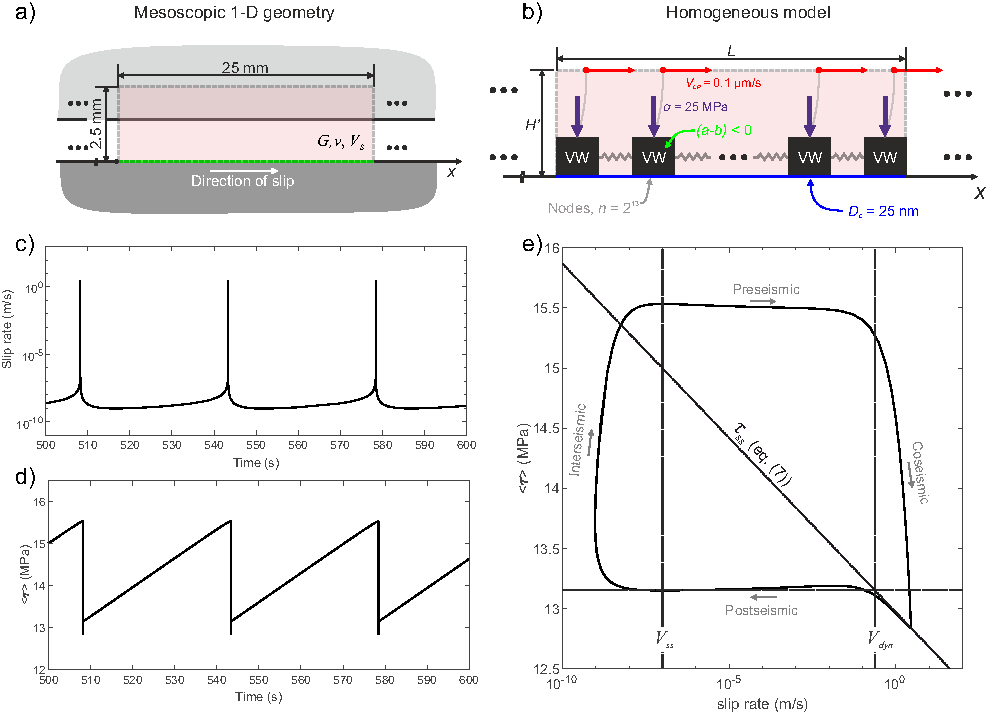
\includegraphics{FIG5_revised.pdf} 
	\caption{\textbf{(a)} General dimensions of the model domain in Figure \ref{fig1}(c). \textbf{(b)} Description of the 1-D boundary value problem being solved by QDYN.  RS frictional behavior is described by equations \eqref{eq5} to \eqref{eq8}. \textbf{(c)} Average slip velocity and \textbf{(d)} average shear stress along the fault for $t_{sim}$ between 500 to 600s. We see that the fault underwent stick-slip behavior. \textbf{(e)} A diagram of the earthquake cycle for the VW fault that includes preseismic, coseismic, postseismic and interseismic phases.}
	\label{fig5}
\end{figure}

Each numerical simulation lasted for $t_{sim}$ = 600 s, which allowed the fault to fully-develop a periodic stick-slip response \citep{Hillers2007}.  Figure \ref{fig5}(c) and (d) show a short time window (500 to 600 s) of the slip velocity and shear stress, respectively, averaged over all nodes in the model.  We see that periodic ruptures are analogous to a `stick-slip' event. Over the full simulation, 18 full rupture stick-slip events were recorded for the homogeneous case but only three are displayed here.  Coseismic slip was defined when any node experienced a sliding velocity $V > V_{dyn}=$0.177 m/s defined by equation \eqref{eq8c}. To further characterize the homogeneous case, Figure \ref{fig5}(e) reveals the relationship between average slip velocity and shear stress, which depicts the seismogenic evolution of the systems between different seismic regimes: interseismic, preseismic, coseismic and postseismic \citep{Ampuero2008}.

\subsection{Heterogeneous $D_{c}$-model}
We produce heterogeneity by varying the distribution of the critical slip weakening distance $D_{c}$ according to the scaling function ($\mathrm{SF}$) in Figure \ref{fig3}(c). The $D_{c}$-model shares some properties of the homogeneous case ($b$ = 0.0144, $a/b$ = 0.65, $\sigma_{n}$ = 25 MPa) and is depicted schematically in Figure \ref{fig6}(a). For the $D_{c}$-model we prescribe the lower value of critical slip weakening distance $D_{c,low}$ = 25 nm. Using the scaling function from the cutting plane method, we can capture the spatial variation in the critical slip weakening distance given as $D_{c}(x) = D_{c,low} \cdot \mathrm{SF}(x)$. Figure \ref{fig6}(b) reveals the spatial fluctuations in $D_{c}(x)$ for heterogeneity on the order of O20. For reference, the spatial distribution of the homogeneous properties are given in Figure \ref{fig6}(c).
 
The average slip rate and shear stress for this $D_{c}$-model (O20) are marked in blue in Figures \ref{fig6}(d) and (e), respectively. For reference, we also depict the results from the homogeneous model O1 (black). We see that the fault experienced stick-slip behavior -- the small spikes in slip velocity -- but did not experience full rupture with a large drop in shear stress drop as in the homogeneous case. 

 \begin{figure}
	\centering
	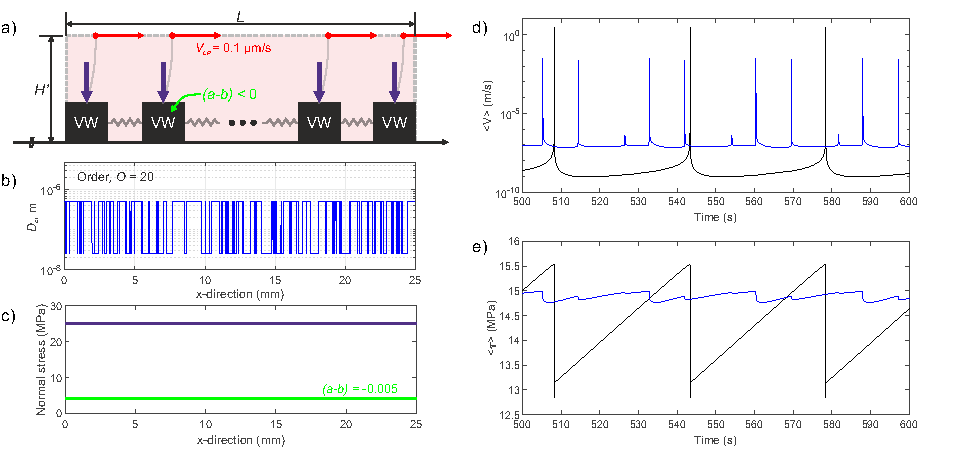
\includegraphics{FIG6_revised.pdf} 
	\caption{\textbf{(a)} General schematic showing the heterogeneous model. \textbf{(b)} Heterogeneous distribution of $D_{c}$, with O20. \textbf{(c)} Constant normal stress and VW rheology ($a-b <$ 0) is shown along the $x$-axis.  \textbf{(d)} Average slip velocity is given along the fault for the heterogeneous model (blue line), which is compared to the homogeneous model (black line). \textbf{(e)} Phase diagram between shear stress and slip velocity for heterogeneous and homogeneous models.}
	\label{fig6}
\end{figure}
 
Next we investigated the effect of different levels of heterogeneity. In Figure \ref{fig7} the average fault behavior is depicted for three levels, O10 (red), O15 (green) and O20 (blue), that all use the same scaling function $\mathrm{SF}(x)$.  This is compared to the average behavior of the homogeneous fault O1 (black).  The average slip, slip rate and shear stress are given in Figures \ref{fig7}(a), (b) and (c), respectively.  We observed an increase in complexity from homogeneity with these models; both O10 (red) and O15 (green) still experienced full system-wide rupture (large events that propagated over the full extent of the modeled fault).  Full rupture nucleated from a smooth section of the fault and did not always arrest when compared to more localized ruptures that occurred in the O20, which had stronger barriers. 

\begin{figure}
	\centering
	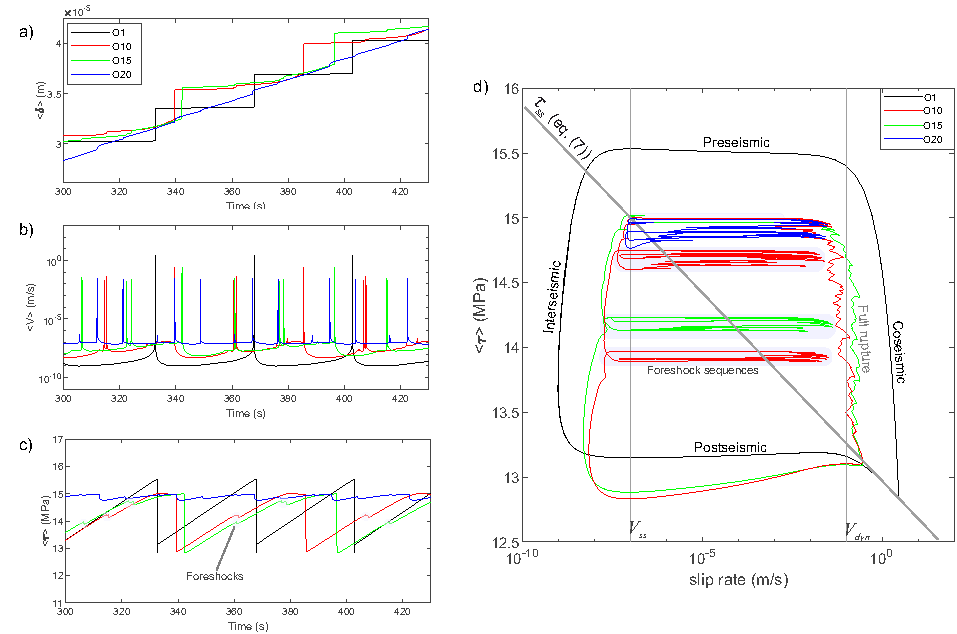
\includegraphics{FIG7.pdf} 
	\caption{Three heterogeneous models $O$ =  10 (red), 15 (green) and 20 (blue) are compared to the homogeneous model (black) for a short time window between 300 and 430 s. We show the \textbf{(a)} average slip, \textbf{(b)} average slip velocity and \textbf{(c)} average shear stress.  We highlight where small drops in shear stress were seen and relate them to small localized events (foreshocks). \textbf{(d)} We examine the phase diagram between shear stress and slip velocity for each heterogeneous model compared to the homogeneous model.}
	\label{fig7}
\end{figure} 

We see that, along with system-wide events, O10 (red) and O15 (green) also experienced small localized events that were arrested by neighbouring barriers. We defined these as ``foreshock sequences'' (discussed later in more detail) leading up to the mesoscopic main rupture (larger stress drop on system-wide events), highlighted in Figure \ref{fig7}(c). We see that as the order O is increased, the fault exhibits transition from well-behaved (homogeneous, O1) to visibly disordered system with full ruptures mixed with small localised ruptures (O10 and O15), then returning to well-behaved, creep-dominated faults with only small localized events on a preferential patch (O20).

To better visualize the system's behavior, we plot all models on phase-diagrams described in Figure \ref{fig5}(e) for the homogeneous case. The average cycles from co- to post- to inter- to pre-seismic behavior, moving around $\tau_{ss}$ in equation \eqref{eq7}. The O10 (red) and O15 (green) models appear to show, in general, lower total stress drops during full rupture events compared to the homogeneous case.  We also see that during a full rupture, the average slip rate on these faults is generally lower than in the homogeneous case.  For the most heterogeneous fault with the order O20, full rupture events did not occur but there was some deviation from steady state caused by small foreshock sequences that prevented the fault from simply `creeping' along at a constant slip rate and steady state shear stress. 

These foreshock sequences are highlighted in phase diagram (gray regions) (Figure \ref{fig7}(d)). Two major sequences were observed for the O10 and O15 models. The timing of these foreshock sequences, relative to the full fault cycle, are presented for O10(red) and occurred in the interseismic stages of the main rupture cycle. For O15(green), one foreshock sequence occurred in the interseismic portion and one occurred soon after the fault entered the nucleation phase of the larger rupture cycle. For O20 (blue), this smooth section of the fault prone to localized rupture behaved in a relative synchronous manner. More details to the spatio-temporal complexity of these ruptures are given in the next section. 

\subsubsection{Spatio-temporal behavior or precursory seismicity }
\label{spatialmodel}

In Figure \ref{fig8} we examine the spatio-temporal evolution of the $D_{c}$-model with O17.5. This model was not presented in the previous section. The purpose of the previous section was to highlight changes in the general fault behavior at three levels of heterogeneity with distinctly different character. All spatio-temporal distributions of slip are depicted in a similar manner to Figure \ref{fig8} in Supplemental Sections S3 for all models.


\begin{figure}
	\centering
	\includegraphics[scale = 0.95]{FIG8_revised.pdf} 
	\caption{\textbf{(a)} Complex rupture for a fault with heterogeneity order $O$ = 17.5. Slip along the fault are given for individual isochrones when the fault was sliding seismically (red, $V_{dyn}>$ 0.177 m/s) or aseismically (blue, $V <$ 0.1m/s).  Results only present simulation times between $t$ = 300 s and 600 s. We use these results to calculate the properties of the localized ruptures that showed local nucleation, dynamic rupture and arrest behavior due to heterogeneity in $D_{c}$. \textbf{(b)} Spatial heterogeneity for a dominant asperity of the fault from $x$ = 5 to 8 mm. \textbf{(c)} A small sequence composed of four individual ruptures between time $t$ = 300 s to 305 s on the dominant asperity. The rupture demonstrates complex distributions of slip and spatio-temporal distributions. To better understand the temporal changes of the rupture, we show the spatio-temporal evolution of Event 4 in terms of its \textbf{(d)} slip velocity and \textbf{(e)} shear stress.}
	\label{fig8}
\end{figure}

Figure \ref{fig8}(a) displays the spatio-temporal evolution of slip along the fault from time $t$ = 300 s to 600 s. The time step between each isochron was uniform, taken every 30 intervals of adaptive time steps.  We note that if any point on the fault slipped rapidly, the adaptive time step would decrease to accurately solve the boundary value problem. Seismicity (red slip isochrones) was defined as any node in the model experiencing slip velocities $V > V_{dyn}=$0.177 m/s. Below this threshold the fault was assumed to slide aseismically (blue slip isochrones). Using this description we clearly identify certain `seismic patches'.

One patch is highlighted in Figure \ref{fig8}(a) and enhanced in (c) where we examine slip on the transect $x$ = 5 to 8 mm from $t$ = 300 s to 305 s.  This asperity section of the fault was prone to seismicity in all models, even the O20 that showed limited localized seismicity and we refer to this as \textit{dominant asperity} from herein. Figure \ref{fig8}(b) demonstrates the spatial variability in heterogeneity in $D_{c}$ along that section (for this case with O17.5). In Figure \ref{fig8}(c), we see that the fault slips aseismically between ruptures, which delineates the seismicity over these five seconds. Four individual ruptures are presented, which exhibited crack-like behavior but remain complex throughout the simulation due to the spatial variability in $D_{c}$, the level of heterogeneity (O17.5) and the continuously evolving shear stress on the fault.

In Figures \ref{fig8}(d) and (e) we investigate the space-time plot of slip velocity and shear stress, respectively, for Event 4 in the asperity failure sequence. The portion of the fault $x$ = 5 to 8 mm is highlighted and we have superimposed the heterogeneity from Figure \ref{fig8}(b) for clarity. We see that Event 4 nucleates at the edge of a `smooth-rough' boundary ($x \sim$ 7.25 mm) depicted as the purple star. As the rupture expands, it propagates bi-laterally at different rates. We have superimposed three lines of constant velocity 0.5$\cdot V_{S}$ (green), $V_{S}$ (red) and $V_{P}$ (blue).  Upon nucleation, the rupture propagates outward in a subsonic manner, moving faster ($\sim 0.75 \cdot V_{S}$) ``up-strike'' into the smoother, less resistive section than into the ``down-strike'', the rougher and more restive section ($\sim 0.45\cdot V_{S}$). This behavior represented typical rupture behavior for localized events on the dominant asperity.

The spatio-temporal rupture evolution for Event 4 is enlarged in Figure \ref{fig9}(d).  Subsonic rupture propagation grows bi-laterally at different rates until arriving at separate barriers. Once the up-strike crack-tip (i.e. that moving on the smooth fault) reached an up-strike barrier, it was abruptly arrested (red star).  As this rupture is arrested a back propagating front is emitted moving closer to the P wave velocity; this front is known as the P stopping phase. This stopping phase was observed by \citet{Madariaga1976} in numerical simulations of kinematic rupture on a circular asperity.  In that problem, the $P$ stopping phase is the wave radiated when the rupture front suddenly haults (red stars), for example when it encounters a strong enough barrier.  Both the up- and down-strike rupture encountered barriers and produced separate $P$ stopping phases.  For the down-strike propagating crack-tip, this $P$ stopping phase actually caused the overall dimension of the rupture to grow larger, eventually terminating at the green star. 

To estimate the properties of each rupture we used an image detection algorithm \citep{Gonzalez2009} and examined the 2-D distance-time space. Using the slip velocity threshold of $V_{dyn}>$ 0.177 m/s, the ruptures were easily separated and the half-length $L_{r}$ is displayed in Figures \ref{fig9}(d).

\subsubsection{Constitutive behavior of individual ruptures }
\label{Constitutive}
One goal of this study is to characterize, compare and validate our RSF model using source properties to those reported by \citet{Selvadurai2019}. We developed tools to quantify the cumulative slip ($\delta$), static stress drop ($\Delta \sigma$), fracture energy ($G^{'}$) and rupture half-length ($L_{r}$) for each rupture to account for their individual complex behavior. In Figure \ref{fig9} we look at the complex behavior of Event 4 from the previous section. Figure \ref{fig9}(d) reveals an enlarged view of Event 4 that ruptured a section with linear rupture dimension $2L_{r}$.  To better understand the complex behavior of all seismic ruptures moving forward, we divide the full length of the rupture into 25 equally-spaced points along the $x$-axis. The number of transects used was sufficient to sample ruptures and to conduct a sensitivity study that investigated the number of required sampling transects (Supplementary Section S2).   

\begin{figure}
	\centering
	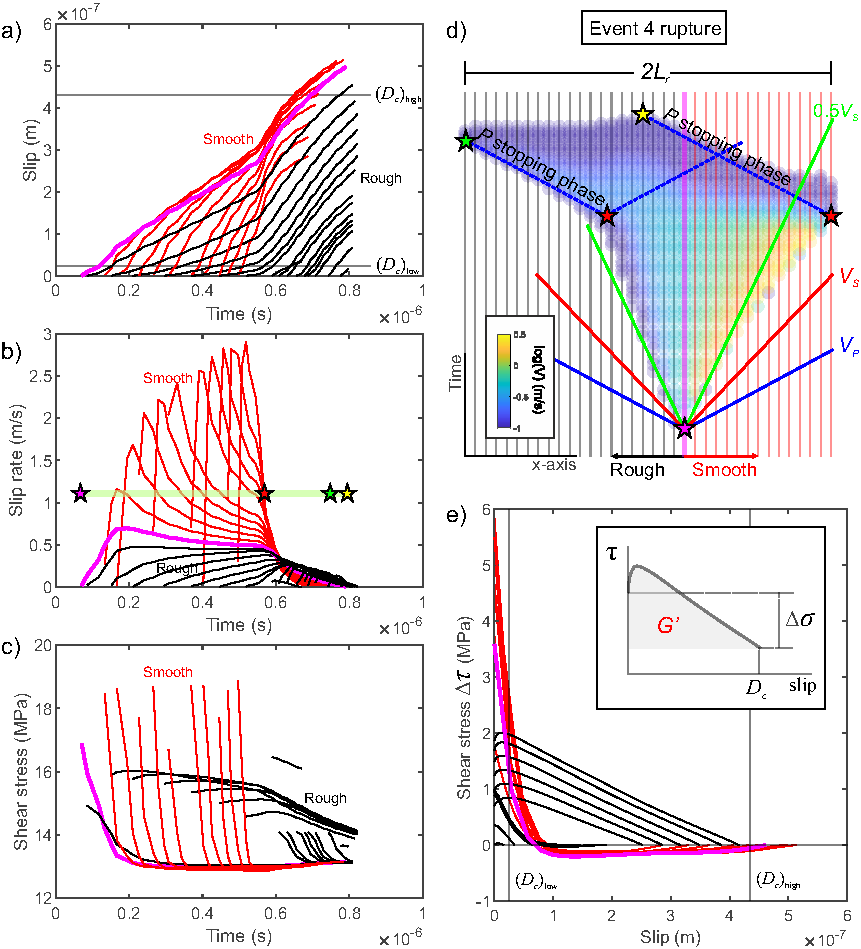
\includegraphics{FIG9_revised.pdf} 
	\caption{Rupture complexity of Event 4 in Figure \ref{fig8}(d) and (e) in space-time plots.  \textbf{(a)} Temporal evolution of slip along 25 different transects of rupture spaced evenly on the fault. \textbf{(b)} Temporal evolution of slip rate along the transects in (a). Key instances of rupture are marked by the colored stars. \textbf{(c)} Temporal evolution of shear stress for the same positions as in (a). \textbf{(d)} Space-time plot of the rupture with the transects depicted graphically. \textbf{(e)} The traction-slip from each transect; the inset image depicts measurements of (static) stress drop ($\Delta\sigma$) and fracture energy ($G^{'}$) for each position on the fault.}
	\label{fig9}
\end{figure}

Figure \ref{fig9} provides a concise temporal understanding of the diversity in the temporal evolution of: (a) slip, (b) slip-rate and (c) shear stress along the spatial transects of Event 4. In Figure \ref{fig9}(a) the rupture has a non-uniform distribution of accumulated slip. The average slip along the 25 estimates was $\delta$ = 0.37 $\mu$m.  We use this to estimate the scalar seismic moment $M_{0}$ given by \citet{Aki1966}: 
\begin{equation}
M_{0} = G A \delta, 
\label{eq9}
\end{equation}
\noindent where $A$ is fault area and $\delta$ is slip. For a penny-shaped fault $A$ = $\pi r^{2}$ and for a square fault $A$ =$(2L_{r})^{2}$. Using this estimate the scalar seismic moment $M_{0}$ = 0.0014 N$\cdot$m. This is equivalent to a moment magnitude $M_{w} = -7.94$.  Transects were color coded for the smooth (red) and rough (black) sections of the fault to highlight differences in dynamic response. As expected, rougher sections showed higher variability in cumulative slip along each transect since they were responsible for arresting the rupture.    

The slip rate along each transect is displayed in Figure \ref{fig9}(b). For further clarity, important times of the rupture are marked by superimposed colored stars. The rupture has higher slip rates along the smoother section of the fault, whereas the rough section offers more resistance with lower slip rates. Shear stress along each transect is presented in Figure \ref{fig9}(c). Smooth portions of the fault (red lines) achieve higher peak stress and exhibit higher weakening rates than the rough sections (black lines), which offer higher resistance to rupture.

Figure \ref{fig9}(e) demonstrates the slip-traction relationship for each transect. Values are normalized with regards to the final stress. Using the inset image we can estimate the (static) stress drop ($\Delta\sigma$) and fracture energy ($G^{'}$).  The latter is sometimes referred to as breakdown work defined by the area under the slip-traction curve\citep[e.g.,][]{Tinti2005, Cocco2016}. We find substantial differences in the participation of each surface (rough and smooth) in the metrics that have be extracted. 

For clarity we have highlighted the critical slip weakening distance for both the smooth $D_{c,low}$ and rough section of the fault $D_{c, high}$. We see that in some cases slip was greater than $D_{c, high}$, which may be explained as dynamic overshoot \citep{Madariaga1976}. Calculating $\Delta \sigma$ is relatively straight forward; to determine the fracture energy $G^{'}$, we numerically integrated the area under this curve. For Event 4, the average static stress drop was $\Delta\sigma$ = 3.25 MPa and average fracture energy $G^{'}$ = 0.13 J/m$^{2}$.  

\subsection{Summary of precursory source properties}
\subsubsection{Seismic moment versus source size}
In Figure \ref{fig10}(a) we examine the relationship between source area $A_{r} = (2\cdot L_{r})^{2}$ and seismic moment $M_{0}$ for the different RSF models. Source properties determined in the previous section are compared to those inferred from seismic waves from an in-depth study by \citet{Selvadurai2019}. We show the results five $D_{c}$-models (circles) against the kinematic estimates detailed by \citet{Selvadurai2019} from P and S waves.  Full ruptures referred to events that ruptured the entire fault surface. RSF ruptures followed the classical empirical scaling relationship between seismic moment and source geometry ($M_{0} \propto L_{r}^{3}$). Figure \ref{fig10}(c) doisplays the relationship between stress drop and seismic moment, which was relatively constant $\sim$ 1.86 MPa where smaller ruptures had slightly lower values of stress drop.

\begin{figure}
	\centering
	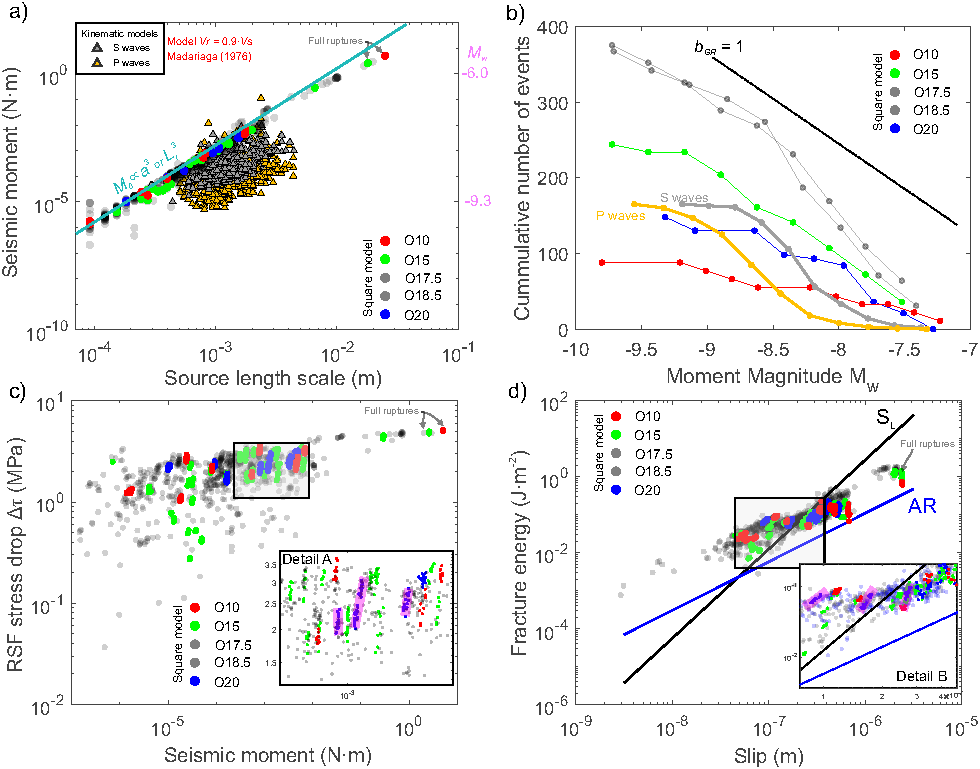
\includegraphics[scale = 0.95]{FIG10_revised.pdf} 
	\caption{\textbf{(a)} Source length calculated from the numerical models with various levels of heterogeneity (colored circles) compared to their scalar seismic moment $M_{0}$. These are compared to the kinematic estimate of source properties determined using shear crack models \citet{Selvadurai2019} for both P and S waves (triangles). \textbf{(b)} Frequency-magnitude distributions (FMDs) are given for each model catalog with $b_{GR}$ = 1 depicted as reference. The inset legend gives the GR parameters: $a_{GR}$, $b_{GR}$ and the magnitude of completeness $M_{c}$. \textbf{(c)} Relationship between stress drop ($\Delta\tau$) and ruptured area $M_{0}$. \textbf{(d)} Fracture energy ($G^{'}$) versus slip. We compare the models to empirical scaling estimates from laboratory seismicity \citep[black line,][]{Selvadurai2019} and extrapolated field estimates \citep[blue line][]{Abercrombie2005}.}
	\label{fig10}
\end{figure}

\subsubsection{Frequency-magnitude distribution}
Estimates of the frequency-magnitude distributions (FMDs) are shown in Figure \ref{fig10}(b). The colors scheme corresponds to Figure \ref{fig10}(a). The Gutenberg-Richter (GR) law describes the magnitude distributions of earthquakes following the standard relationship $log_{10}(N)= a_{GR} - b_{GR}M_{w}$, where $N$ is the number of events equal to or above magnitude $M_{w}$ and $a_{GR}$ and $b_{GR}$ are constants describing the productivity and sizes of earthquakes, respectively\cite[e.g.][]{Wiemer2002}.  

The legend gives the maximum likelihood estimate of the $a_{GR}$- and $b_{GR}$-values computed based on events above the magnitude of complete recording $M_{c}$ \citep{Wiemer2002}. Typically $M_{c}$ is used to asses the completeness of the catalog under investigation, i.e. above which magnitude does the GR law fits the data best. We note that the nature of the GR relationship is scale-invariant and in our model, where all events can be recorded without converge bias, the completeness magnitude $M_{c}$ is related to physical effect discussed in Section \ref{EffectsFMD}. As the order of heterogeneity increases $a_{GR}$- and $b_{GR}$-values. Lower $b_{GR}$ were observed on stick-slip dominant fault (O10 and O15) and increased on creeping faults (O20).

\subsubsection{Fracture energy scaling}
\label{FracEnergy}
Scaling behavior between fracture energy $G^{'}$ and slip $\delta$  is compared to the  empirical relationship $G^{'} \propto \delta^{\gamma}$. In Figure \ref{fig10}(d) estimates of $G^{'}$ for the different models are presented. These are compared to the previously discussed empirical relationship for shear crack source models from laboratory experiments ($S_{L}$, $\gamma = $2.35) \citep{Selvadurai2019}  and estimates made at regional scales from natural earthquakes (AR, $\gamma = $1.28) following the observations of \citet{Abercrombie2005} \citep[see also][]{Mai2006}.  We see that the results from the model tend to follow the same slope as AR but, if we look more closely, at Detail B in Figure \ref{fig10}(d), we see that some of the smooth patches show steeper trends in scaling. This can be explained by the fact that the preferential worn patches remain relatively constant in size but the stress drop varies, as depicted in Detail A of Figure \ref{fig10}(c).

\subsubsection{Creeping to stick-slip transition}
\label{Recurrence times}
Figure \ref{fig11} marks the average slip (black) and average shear stress (red) for 100 s of the simulations for strong barriers O20 (left-hand side, LHS) to weaker barriers O10 (right-hand side, RHS) and the transitional case O17.5 (middle panel). The general behavior of the fault transitioned from creep-dominated (O20) to stick-slip dominated (O10). Creep-dominated and stick-slip dominated are defined by how much the average slip deviates from the creep rate ($V_{creep} = t\cdot V_{LP}$). This transition from creep- to stick-slip-dominant behavior occurred as the level of heterogeneity was decreased. In all simulations, the fault was driven at a constant loading rate and its impact on the general behavior is the subject of future work.  Figure \ref{fig11} highlights the distinct regimes and the appearance of foreshocks in a broad sense \citep{Mogi1985} are discussed in Sections \ref{Cascade_UP} and \ref{Dominant}.

%Next we examine the recurrence rate $T_{r}$ for localized events in each model, which is considered to be the time between any two events at any location on the fault. To differentiate triggered  seismicity (e.g. aftershock) from isolated events, we adopt the methodology described in \citet{Lengline2009}, who looked at the probability distribution function (PDF) of the recurrence times normalized by the average recurrence time $T^{*}_{r}$.  They found that events below $T_{r}/T^{*}_{r} <$ 0.1 follow a power-law distribution consistent with Omori's law that describes aftershocks in nature \citep[e.g.,][]{Lengline2009}. 

%In Figure \ref{fig11}(b) we show the probability distribution of $T_{r}/T^{*}_{r}$ for the five $D_{c}$-models. The purple region highlights portions of the distribution that are not considered to be triggered events according to \citet{Lengline2009}. We see that for the creep-dominated O20 model there is almost equal probability in recurrence time but a slight increase in  $T_{r}/T^{*}_{r} >$ 0.1 promoting the conjecture that these events are not triggered but are the result of the overall aseismic loading of the fault. In the transitional models (O18.5, O17.5 and O15) we fit a power law distribution (gray lines) between 1e-5 $< T_{r}/T^{*}_{r} <$ 0.1 and found its slope to decrease as heterogeneity was decreased. We note a small `bump' in probability above $T_{r}/T^{*}_{r} >$ 0.1, denoted with the small arrow in O15. This appears to have been amplified in O10, or the stick-slip dominated model, discussed later in conjunction with the results surrounding the FMDs.  This may be related to cascade-up foreshock behavior (see Discussion Section \ref{Cascade_UP}) but requires more rigorous investigation beyond the scope of the current study.

\begin{figure}
    	\centering
	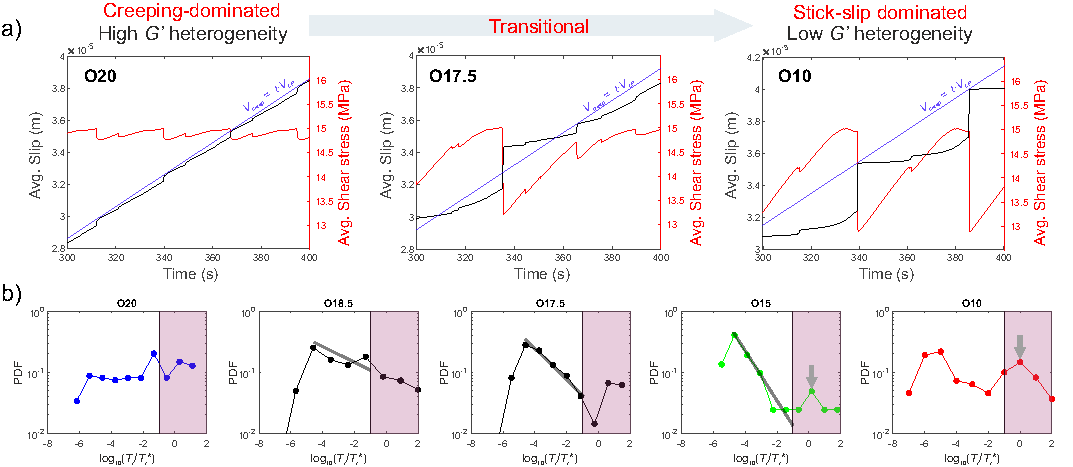
\includegraphics[scale = 0.9]{FIG11_revised.pdf} 
	\caption{Earthquake recurrence rate for each $D_{c}$-model from higher O20 to lower O10 levels of strength heterogeneity. (\textbf{a}) The average behavior of the entire fault for small portions of time $t$ =300 to 400 s for the O20 (creeping-dominated), O17.5 (transitional) and O10 (stick-slip dominated) models. (\textbf{b}) Probability distribution functions of the lognormal distribution of normalized recurrence rates $T_{r}/T^{*}_{r}$ for all models. The probabilities above $T_{r}/T^{*}_{r} >$ 0.1 in purple are highlighted.}
	\label{fig11}
\end{figure}

\subsection{Heterogeneous \textit{Composite}-model}
The primary goal of this study is to provide an understanding of what types of RSF heterogeneity may explain a suite of experimental observations. Prior models have employed heterogeneity with a minimal level of unknown variables. We increase the complexity of the model using a \ital{Composite}-model; this model aims to illuminate any additional complexity that may exist in the spatial distribution of normal stress. This model is presented to expand the possible boundary conditions that can feasibly explain the concomitant slow and fast slip on a frictional interface. 

We use measurements from the pressure sensitive film (Figure \ref{fig4}(b)) to implement variability in normal stress. More information on the pressure sensitive film is given in \citet{Selvadurai2017}. We use the scaling function where on smooth sections (low $D_{c}$) we prescribe constant normal stress $\sigma_{n, high}$ = 25 MPa and on rough sections, we apply a constant low normal stress level, set to the lower measurable limit of the pressure sensitive film $\sigma_{n, low}$ = 12 MPa \citep{Selvadurai2015a}. 

Figure \ref{fig12}(a) depicts a section of the spatial heterogeneity on the dominant asperity under normal stress $\sigma_{n}$ (red) and at a critical slip weakening distance $D_{c}$ (blue).  The scaling function was chosen to be O20, a model that previously had a relatively well-behaved response.  We use the same methods to calculate source properties and examine similar relationships for this composite-model (O20C).

\begin{figure}
	\centering
	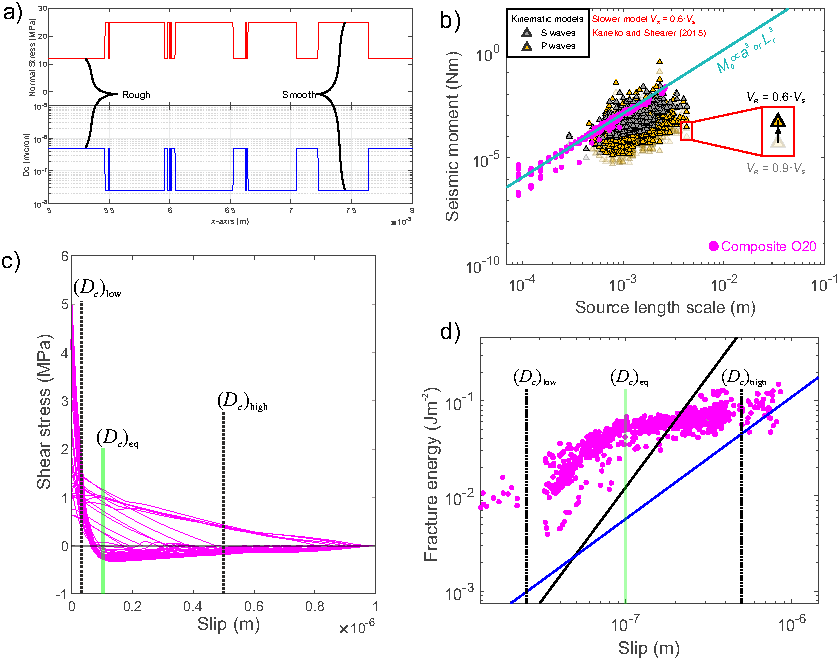
\includegraphics{FIG12_revised.pdf} 
	\caption{Results from the \textit{Composite}-model. \textbf{(a)} A small section of the 1D fault from $x$ = 5 to 8 mm showing the spatial variation in both $D_{c}$ and $\sigma_{n}$. \textbf{(b)} The scaling relationship between $A_{r}$ and $M_{0}$ (gray circles) is compared to the corrected kinematic estimates of source properties from \citet{Selvadurai2019} (triangles).   \textbf{(c)} Constitutive behavior for a large event in the \textit{Composite}-model. \textbf{(d)} Relationship between fracture energy $G'$ and slip $\delta$. Empirical relationship between black and blue lines is similar to that demonstrated in Figure \ref{fig10}(d).}
	\label{fig12}
\end{figure}

Figure \ref{fig12}(b) reveals the relationship between $M_{0}$ and $A_{r}$, with similar estimates as the kinematic shear crack model in Figure \ref{fig10}(a). However, here we have made additional assumptions in the shear crack model regarding rupture speed.  We apply a correction factor to account for slower ruptures in kinematic models, for example $V_{r} = 0.6\cdot V_{S}$.  This analysis was performed by \citet{Kaneko2015} for a range of rupture scenarios: circular or elliptical and symmetric or asymmetric.  They found that decreasing the rupture speed can produce deviations of up to 2.5 times higher in terms of stress drop depending on the model and the wave phase (P or S).  Average RSF estimates of rupture velocities were much lower 0.6$\cdot V_{S}$.  From Table 1 in \citet{Kaneko2015}, we updated the estimates from \citet{Selvadurai2019}, which minimized the difference between the kinematic (triangles) and RSF (circles) estimates of source properties.  Original kinematic estimates are scaled by those from an asymmetric circular asperity model with rupture velocity $0.6\cdot V_{S}$ leading to an increase in seismic moment by 2.63 for P wave estimates and 2.74 for S waves estimates.

Figure \ref{fig12}(c) displays the constitutive shear stress versus slip behaviour for a large random asperity. For reference, we mark the levels of $D_{c,low}$, $D_{c,eq}$ and $D_{c, high}$.  The term $D_{c,eq}$, or equivalent critical slip weakening distance, appears to be a representative critical slip weakening distance that always lies between the two $D_{c}$ limits but will likely vary for each rupture as a function of the ratio of high to low resistance of the interface participating in rupture. Looking at the relationship between $G^{'}$ and slip, we see that it appears to have a ``kink''.  This kink is observed at about the slip level of $D_{c,eq}$. 

\section{Discussion}
We have summarized findings from a well-documented laboratory experiment \citep{Selvadurai2015, Selvadurai2017, Selvadurai2019} that displayed complex nucleation behavior: preparatory slow preslip accompanied by intermittent localized seismicity from the same sections of the frictional interface (see Figure \ref{fig1}). A RSF model was developed to examine the complex frictional behavior using the rate- and state-dependent constitutive framework. The model accounted for wear observed from \textit{a posteriori} measurements of roughness on the slider block surface that was well characterized in terms of a bimodal Gaussian distribution of surface roughness (Figure \ref{fig2}(a)). Attributes of our worn interface show a distinct polished surface embedded in a rougher surface, a feature that may be similar to the polished fault mirrors (FMs) observed on natural outcrops (see Figures \ref{fig2}(e) and (f)).

A cutting plane method (Figure \ref{fig3}) was used to mathematically quantify the spatial variation between smooth and rough sections. Two sets of RSF properties were chosen based on the fact that smooth surfaces have lower critical slip weakening distance $D_{c}$ than rougher sections and the level of heterogeneity was investigated. The models showed complex behaviour (Figure \ref{fig7}) that differed from the homogeneous case (Figure \ref{fig5}); this could explain the experimental observation of concomitant slow slip and localized seismicity.  We developed algorithms to isolate ruptures (Figures \ref{fig8} and \ref{fig9}).  These allowed us to estimate a range of source properties, such as scalar seismic moment ($M_{0}$), rupture length scale ($L_{r}$), seismic slip ($\delta$), stress drop ($\Delta\tau$), fracture energy ($G'$), frequency-magnitude distributions (FMD) and recurrence rates ($T_{r}$) of five different $D_{c}$-models and a composite-model (Figures \ref{fig10}, \ref{fig11} and \ref{fig12}). These calculations were compared to independently estimated seismological source properties made from interpretation of the seismic waves \citep{Selvadurai2019}.

\subsection{`Cascade-up' nucleation behavior}
\label{Cascade_UP}
Our model exhibits a wide range of behaviors, ranging from relatively simple to chaotic (see Figure \ref{fig7}). In Figure \ref{fig5} we observe that homogeneous rupture is well-behaved, exhibiting regular stick-slip events at a constant recurrence time.  In the model, we assume periodic boundary conditions. This implies that if a rupture is not arrested in the mesoscopic region and reaches the boundary it would theoretically continue to rupture the macroscopic region -- cascading-up and creating a system-wide stick-slip event that was observed experimentally (Figure \ref{fig1}(b)). 

We referred to these events as full-ruptures and these are linked to cascade-up nucleation processes. This assumption is plausible when looking at the hypocenter of the full-fault rupture (i.e. system-wide stick-slip event) measured experimentally in \citet{Selvadurai2015}. These were consistently located in the region near the roughness measurement \citep[magenta star in Fig. 7 and 8 in ][]{Selvadurai2015}. In Figure \ref{fig11}, the two types of end-member behaviors are highlighted: 'creep dominated' and 'stick-slip dominated'. Stick-slip dominated behavior is described as supporting localized foreshocks but also small events would cascade-up and trigger full ruptures. The creep dominated events form the O20 model were localized but they never developed into full ruptures. The $D_{c}$-models O10 and O15 exhibited foreshock sequences that were followed by a cascade-up into full ruptures (Figure \ref{fig5}), whereas O20 showed constrained ruptures that did not cascade-up. 

Both the O10 and O20 models had identical level of normal stress $\sigma_{n}$ leading to similar levels of peak and residual shear stress levels but the variations in $D_{c}$ imposed differences in the weakening rates and fracture energy on the rough sections of each model. Therefore the order of the model was directly related to the the level of heterogeneity in fracture energy for our models. We found that for relatively low levels of fracture energy heterogeneity faults displayed a stick-slip-dominant behavior (foreshocks that can potentially cascade-up) and, once the heterogeneity is large enough, a creep-dominant behavior is observed. Hierarchical heterogeneity in fracture energy has been proposed by others \citep{Ide2005, Aochi2014, Aochi2017} and will be discussed later.

While we cannot confirm an exact wear mechanism that may produce flat sections or increase the level of heterogeneity between smooth and rough sections, one hypothesis is that certain sections of the fault are more prone to flattening (ironing) and others will develop particles of gouge. Flattening, or ‘ironing’, of asperities due to adhesive wear has recently been investigated using a material independent framework \citep{Aghababaei2016}. Physics-based numerical simulations found a critical length scale describing the deformation mechanisms of interacting asperities. At length scales below a critical value, asperities flatten inelastically, dependent on the size of the asperity junction, the work of adhesion of the bulk material, and the maximum elastic strain energy that can be stored at a contact. This explanation fits observations made by \citet{Siman-Tov2013} and others that studied fault mirror formation in the laboratory. \citet{Brown1986} found that flattened patches could form upon the closure the interface indicating significant  plastic flow at the highest points on the surface, albeit at smaller length scales than mirror surfaces studied and produced in the laboratory \citep{Fondriest2013,Siman-Tov2013, Tisato2012,Siman-Tov2015}.

\subsection{Dominant asperity}
\label{Dominant}
All models hinged about the behavior of specific section of the fault from $x$ = 5 mm to 8 mm, we referred to as the dominant asperity (Figure \ref{fig8}(b) and (c)). In all models, this section produced localized events. With lower levels of heterogeneity (O10 and O15) both foreshocks and events that cascaded-up were produced, rupturing the whole fault. In Supplemental Sections S3, we show spatio-temporal evolution of slip of O10 and the O15 full-ruptures, which breakdown in a similar manner -- nucleating each time from the dominant asperity.

This type of behavior may explain the observations in the Naka-Oki region in eastern Japan \citep{Okuda2018} and the Tohoku–Hokkaido subduction zone, Japan \citep{Ide2019}. Where earthquakes shared almost identical growth offering patterns for repeating events of various sizes. This observation appears to be consistent with our model, an explanation that repeater asperities that routinely produce  $M_{w} \sim$ 2 could have lower values of fracture energy (or $D_{c}$) that sometimes cascade-up to  $M_{w} \sim$ 4.8 \citep{Okuda2018a}.  These authors hypothesize that a hierarchical structure exists \citep[as depicted in fig. 5 of ][]{Okuda2018}, possibly due to heterogeneity in the fracture energy \citep{Ide2005, Aochi2014, Aochi2017}. Our model agrees with this hypothesis and heterogeneity in fracutre energy is provided in the form of polished smooth sections in a rougher interface. 

%Using the \citet{Eshelby1957} penny-shaped stress drop model in a Poissonian material, we can estimate the source radius as $a_{r} = \sqrt[3]{(7/16)(M_{0}/\Delta\sigma)}$, for an $M_{w}$ = 2. If we assume stress drops between $\Delta \sigma  = $ 1 MPa and 10 MPa, we find that the source radius varies between $a_{r}$ = 36.5 m and 78.5 m.  While these seem to be very large, there have been cases of such large exposures of FMs on outcrops of normal faults in central Greece \citep{Jackson1999}. These sizes of these FMs could explain the smaller $M_{w}$ = 2 repeater events in the Naka-Oki region of Japan.  

We also observe interesting behavior surrounding the unlocking sequence of the dominant asperity in Figure \ref{fig8}(c). For clarity, the temporal unlocking sequence for the O17.5 model were enumerated in ascending order from 1 to 4.  Below the spatio-temporal slip evolution (red and blue isochrons), we show the spatial length of each rupture. We can see that each rupture overlaps the previous rupture, a phenomenon was also observed by \citet{Okuda2018a} and referred to as 'streaking', which they claimed explained the patches of differing sizes possessing some hierarchical structure. This also might be similar to the dynamic precursor detachment fronts observed experimentally on fault analogs \citep{Rubinstein2004,Rubinstein2006} and the breakdown fronts seen on granite-granite interfaces by \citep{Ke2018}. \citet{Okuda2018a} attribute this specific rupture process to subtle differences in the physical conditions of the fault interface, which appear to be consistent with a fault interface consisting of a series of hierarchical structures. Our model produced foreshocks in a broad sense \citep{Mogi1985} and was due to the patchy distribution of fracture energy on the smooth/rough idealization.

\subsection{Repeating-like behavior}
In contrast to the cascade-up behavior discussed above, the dominant asperity ($x$ = 5 mm to 8 mm) also showed quite regular behavior when the level of heterogeneity was increased to O20.  Spatio-temporal evolution of slip from 300 s to 600 s for the O20 model is also given in Supplemental Section S3. For this model, the average shear stress and slip rates remained near steady state (equation \eqref{eq7}) and the only deviation came from the local increase in slip rate during ruptures of the dominant asperity.  In Figure \ref{fig11} we refer to this as `creep-dominated'. For our creep-dominated fault, any event produced by the dominant asperity was easily arrested by the rougher surroundings, which in the model, were actually regions exhibiting relatively larger fracture energy.  This `creep-dominated' behavior is similar to that observed for repeating earthquakes in nature \citep[e.g., ][]{Beeler2001,Uchida2019}

Models used to understand repeating earthquakes typically involve a circular asperity embedded on a planar fault, where the asperity is relatively locked with respect to the creeping region that loads a resistive asperity. When studied using RSF laws, the creeping region is typically given velocity-strengthening (VS, $a-b>0$) properties and the asperity is velocity-weakening  (VS, $a-b<0$) \citep{Kato2003,Chen2009}. In these models, seismicity can only occur on the VW asperity and their ability to trigger more complex behavior, e.g. a cascade-up style rupture, cannot exist unless additional VW regions are specified. \citet{Noda2013} looked at the behavior of smaller VW asperities embedded on a larger VW asperity while varying ratios of RSF properties and found very complex model behavior. Our model finds that, due to the heterogeneity the in polished-to-rough surface, we can actually host constrained earthquakes in an entirely VW region that depends on the level of heterogeneity.  As heterogeneity increases between the polished and rough sections, repeating events and creep-dominated behavior may become more apparent.  A hypothesis for the wearing mechanism that may explain the continued increase in strength heterogeneity is offered in Section \ref{Cascade_UP} and focuses around the numerical modeling of wear by \citet{Aghababaei2016}.

\subsection{Crack-like ruptures}
Figures \ref{fig8}(d) and  (e) summarized the behavior of a crack-like rupture typically seen on the dominant asperity. Nucleation of the precursory events mostly occurred on the boundaries between the smooth-rough transition on the VW interface. This type of behavior has been observed in a larger scale 2D RSF simulation of the Parkfield section of the San Andreas Fault, CA, USA \citep{Barbot2012}, in conceptual models of interacting asperities \citep{Kato2003} and complex megathrust subduction zones \citep{Kaneko2010}; however, nucleation in these models is always at a VS-VW transition. 

From Figure \ref{fig9}, we see that the smoother ruptures were more efficient, reaching higher slip rates, having higher stress drop and producing less fracture energy. Slower rupture speeds coupled with less stress drop and higher fracture energies occurred on sections that had a ``rough'' parameterization, which was as expected.  The complex interaction of how the rupture that propagated on both a polished and rough interface was apparent even as it decelerated, when the P waves stopping phase was observed \citep{Madariaga1976}. This stopping phase appears to be reflected or emanating from the smooth-rough boundaries. 

In general, these localized ruptures appear to follow larger scale laboratory experiments that studied rupture propagation on pre-cut granite-granite \citep{Passelegue2013} and similar experiments on a direct shear PMMA-PMMA friction apparatus \citep{Rubinstein2004,Rubinstein2006,Ben-David2010, Fineberg2015,Svetlizky2014}. In the literature, we could not find details into surface preparation techniques or any indication of their RMS roughness in these authors complimentary experiments. However, if their interface was nanometrically smooth throughout its entirety, it promote homogeneity of frictional properties. Selvadurai and Glaser (2017) found that nanometrically smooth roughness ($\sim$ 22 nm RMS) was measured on multiple polished/worn sections. For both independent studies transition from quasi-static to dynamic rupture might have occurred at similar length scales, controlled by this (very smooth) roughness. The differences between the observation is (1) our ruptures arrested locally on millimetric scales (due to heterogeneity) and (2) theirs continued to rupture the entire fault (due to homogeneity). \citet{Svetlizky2014} observed crack-like Mode II ruptures that propagated over their entire fault. Our model also predicts this behavior for the homogeneous model (Figure \ref{fig5}) but explain why heterogeneity is needed to arrest ruptures and generate foreshock seismicity in our RSF.

These studies looked at dynamic rupture propagation in the framework of fracture mechanics with slip-weakening friction \citep{Ida1972,Andrews1976,Kammer2012,Kammer2015}.  As discovered by \citet{Cocco2002}, RSF can reproduce slip-weakening behavior. We see from constitutive behaviors describing the $D_{c}$  and composite models, respectively, Figures \ref{fig9}(e) and \ref{fig12}(d), that dynamic weakening effects are minimal. This appears to open up future investigations into precursory events using dynamic fracture mechanics as an alternative to the RSF presented here.

\subsection{Dynamic RSF source properties}
The model displays great complexity at the mesoscopically (Figure \ref{fig7}) and microscopically scales (Figures \ref{fig8} and \ref{fig9}). Dynamic RSF source estimates of moment to source length scale followed the standard $M_{0} \propto L^{3}_{r}$ , which also matched kinematic estimates in \citet{Selvadurai2019}. While the dynamic and kinematic source estimates highlighted here differ slightly, the magnitude and trends between estimates are similar even though the problem is approached from two different modeling frameworks. Comparing these two different models is an important step towards validating the effectiveness of each model and understanding how to link precursory seismicity to the nucleation phase on fault analogs. Identical validation efforts have been used for RSF models looking at repeating earthquakes in Parkfield, CA \citep{Chen2009}.

Stress drop is dependent on the rupture velocity ($V_{r}$) \citep{Kaneko2015}. We found our crack-like rupture to be much slower (0.6$\cdot V_{S}$) than those typically used in kinematic approaches, where kinematic shear crack models assume rupture velocities between 0.9 and 1.0$\cdot V_{S}$ \citep{Cocco2016, Selvadurai2019}. With this additional knowledge, updates to our original kinematic estimates were made by applying correction factors from numerical studies performed by \citet{Kaneko2015}. This correction factor increased the correlation between kinematic estimates and RSF estimates. Using more accurate estimates of rupture velocity when estimating source features via kinematic crack-models should be done carefully and investigated in more detail \citep{McGuire2018}.

Fracture energy $G^{'}$ versus slip was compared for two types of model ($D_{c}$ and composite) with scaling relationships in the lab ($S_{L}$) and field ($AR$). The $D_{c}$ model followed the $AR$ scaling relationship more closely, which we attribute to the fact that ruptures occurred with the rougher (more resistive) portions more than in the composite model.  Perhaps this was due to the description of heterogeneity in the models. The $D_{c}$-model had a constant shear strength and, therefore, heterogeneity in both the slip-weakening rate and fracture energy on the polished/rough sections controlled the source properties. The Composite-model added to the complexity by including normal stress variability, causing an additional heterogeneity in the shear strength of the fault (see equation \eqref{eq5}). This additional complexity caused more localized seismicity that occurred because of larger contrasts in slip-weakening rate and less contrast in the fracture energy between the polished and rough sections. This is clearly seen in the O20 and O20-C spatio-temporal distributions of slip that shown in detail in Supplemental Figures S3.4 and S3.5, respectively. The composite model nucleated more events but, similar to the less complex model, there was no cascade-up rupture.  In the composite model, geometrically smaller smooth sections could nucleate rupture but they would arrest due to the lower strength of the rough region. The purpose of this study was to provide a reasonable parameter space (Figure \ref{fig4}) based on a suite of experiments that, when combined with a novel RSF model, provides insight into the potential behaviors of worn faults in nature.

\subsection{Effect of fracture energy heterogeneity on FMDs}
\label{EffectsFMD}
Analysis of the FMDs showed that creeping faults (O20 and O20-c) had higher $b_{GR}$- and $a_{GR}$-values than stick-slip dominant faults (O-10 and O15). A gradual transition was observed from both low to high $a_{GR}$- and $b_{GR}$-values as the heterogeneity in fracture energy was increased. This observation follows studies in natural tectonic settings where creeping sections were found to have higher b-values than locked section prone to larger earthquake \citep{Amelung1997, Tormann2014}. \citet{Goebel2013} found that temporal decreases in laboratory estimates of b-values occurred moments leading up to larger stick-slip events, a phenomena that has been observed in natural tectonic settings prior to large megathrust events \citep{Tormann2015,Gulia2016,Gulia2019}. Our model suggests that lower b-values may occur on faults that also experience foreshock behavior and both observations can be reconciled by a hierarchical structure of the fault that exhibits low (but distinct) variations in fracture energy distribution.

\citet{Dublachet2013} modeled various densities of velocity weakening asperities surrounded by creeping velocity strengthening using a 3-D continuous quasi-dynamic rate-and-state model. They were able to generate reasonable Gutenberg-Richter statistics by dynamic cascades of events which differed from our model. While cascading event were observed as shown by sequences with normalized recurrence times $T_{r}/T^{*}_{r}$ below 0.1, we also observed individual events that were decoupled from cascading features ($T_{r}/T^{*}_{r} >$ 0.1). 

Completeness in our model is associated with the minimum size of resolvable earthquake defined by the mesh scheme and solution convergence (Supplemental Section S1). This differs from the field where $M_{c}$ is affected by the fact that the recording network is only capable of recording a fraction of all events for magnitudes smaller \citep{Wiemer2002}. By definition, the Gutenberg-Richter law is scale-invariant above the magnitude of the completeness threshold ($M_{c}$). Below this threshold, the size and occurrence of seismicity is scale-variant. While scale-invariant is produced by our model, a large number of events fall below this threshold and are likely due to the scale-variant mechanism associated with the smoothing of high asperities during the wearing process. More extensive studies will be needed but we note these features had important impact on important nucleation physics, such as foreshocks and cascade-up style failure, that may be useful to earthquake forescasting and prediction. From a statistical perspective, events falling below $M_{c}$ are not used and using more involved methods that investigate the catalog behavior near and below $M_{c}$ will be useful \citep{Mignan2012, Mignan2020}.

%\subsection{RSF is a phenomenological tool}
%A major focus of this study was to quantify the seismic RSF source properties independently from the kinematic estimates made using seismic source models inferred from high-frequency ground motions \citep{Selvadurai2019}. This is in important exercise to check the validity of the model. As noted earlier, RSF is a phenomenological approach to understanding complex frictional processes.  It has been successfully used to capture a number of controlling features in frictional behavior, such as the micro-mechanics associated with dry contact on rough and smooth interfaces \citep{Marone1998,Yoshioka1997} and the shear banding (B and Y planes) along gouge-rich interfaces with different particle sizes and shapes \citep{Marone1993, Anthony2005,Scuderi2017}. While it may seem trivial to validate aspects of the model in scaled laboratory experiment, this is necessary to ensure that the model performs in an acceptable manner when scrutinized by more rigorous experimental data.

%Recent experimental studies cross-validated using the RSF model have showed that the existence of the expanding preslip nucleation region  \citep{Nielsen2010,Kaneko2011} and the effect of normal stress on the critical nucleation size \citep{Latour2013,Kaneko2016}. These types of studies accomplish three objectives: (1) Posit an understanding of boundary conditions that is plausibly explained with the applied friction law, (2) validate the theoretical predictions of frictional behavior in the model \citep{Ruina1983,Rubin2005,Ampuero2008} and (3) estimate frictional parameters that are not easily up-scaled to field scenarios. Our study expands on these points and provides a model that matches additional experimental observations (precursory/foreshock seismicity) within the nucleation zone. Moreover, our description of geometric heterogeneity is defined through an experimental manner (cutting plane methods), which further embodies the phenomenology that is intrinsically embedded in RSF.

\subsection{Prescribing heterogeneity on velocity weakening faults}
In Section \ref{SurfaceWear}, we highlighted findings from tribology in which wearing of surfaces can produce nanometrically smooth regions in an overriding rougher surface that is well-characterized by the bi-modal Gaussian PDF of surface height. These polished sections have also been linked to fault mirrors through laboratory tests under a range of conditions (slow and fast sliding and at high-temperature). Laboratory experiments give explanations as to why these FMs exist on exposed outcrops but do not give the extent of how large they may grow due to constraints of typical laboratory studies that produce them. Unfortunately, our understanding of polished fault mirrors from exposed outcrops is constrained by our ability to observe them; an obvious limitation exists when we compared the volume of exposed outcrops to the volume of active faults producing seismicity in nature.  

Our model suggests that the scale of polished sections to rough sections is important; correspondingly, we conjecture that attempting to capture this using the single fractal measurement of the Hurst exponent is not adequate (the scale at which needs more investigation). Since the mirrors in our model required a bi-modal Gaussian distribution of surface heights, new research into fractal characterization of such surfaces by \citet{Hu2019} suggests that a bi-fractal distribution in roughness is more representative \citep{Leefe1998, Pawlus2008}. These surfaces have already been shown to influence characteristics of acoustic emission energy release upon sliding \citep{Fan2010, Hu2019a} but these results are recent and more investigation is required. Bi-modal Gaussian and b--fractal stochastic descriptions of frictional parameters may help us understand complex frictional behavior, such nucleation dynamics with foreshocks without large assumptions imposed by the modeler.

\section{Conclusions}
We developed RSF to capture slow aseismic transients coupled with localized foreshocks and compared this to similar behavior observed in a concerted laboratory experiment on a fault analog. Heterogeneity was necessary and prescribed using the worn surface roughness that displayed a bimodal Gaussian distribution of surface heights. We discretized smooth and rough faults using an understanding the micro-mechanics of the critical slip $D_{c}$ where smooth sections have lower values. This resulted in polished sections (mirrors) producing small ruptures, whereas rougher sections hosted aseismic slip.  

The behavior of the fault varied between creep-like to stick-slip dominated and depended on the level of heterogeneity in the fracture energy. Small localized events were particularly interesting around a dominant asperity that produced seismicity in every simulation and appeared to control cascade-up-breakdown of the fault when the level of fracture energy heterogeneity was low. 

Seismic source properties were validated against independent kinematic estimates from elastodynamic ground motions. Rupture velocity obtained from the RSF models estimated that subsonic ruptures propagated at speeds close to $V_r = 0.6\cdot V_{S}$.  This was used to adjust kinematicsource properties by \citet{Selvadurai2019} for the slower crack-like ruptures. Validating the RSF source properties was deemed sufficient for a first-order understanding of the modeled frictional heterogeneity that may explain simultaneous foreshocks and aseismic preslip. We believe that this should be further explored in more robust parametric studies. 

Worn faults observed in nature have the form of fault mirrors but it is unclear how they truly evolve over geologic time, their spatial extent and how this evolution affects the frictional response of a shear principal slip zone. In our wear-based model, changes in the level of heterogeneity in fracture energy caused end-member behavior from creep to stick-slip dominant. Future experiments will need to investigate this behavioral evolution and potentially update the stochastic descriptions of frictional parameters on faults that contain FMs. 

%\acknowledgments
\section*{Acknowledgments}
We would like to thank T. Yamaguchi, L. Villiger, B. Edwards T. Tormann, P. Bhattacharya and A. Mignan who provided important discussion points regarding the analysis. Key insights into simulations presented here are given by J.-P. Ampuero. This research was supported by: JSPS KAKENHI Grant Number JP16H06478 in Scientific Research on Innovative Areas ``Science of Slow Earthquakes''. Computational resources were provided by the Information Technology Division and Extreme Computing Research Center (ECRC) at KAUST. Funding for parts of this research was provided by the National Science Foundation Grant CMMI‐1131582 awarded to SDG at the University of California, Berkeley. Funding for PAS was provided through the OFES Project: EDGAR ‐ Dimensionnement du réseau de fractures dans les réservoirs géothermaux (Contract SI/501495‐01). PMM's contribution to this study and a research visit of PAS to KAUST was supported by KAUST research grant BAS/1/1339-01-01. Finally, the authors assume full responsibility for the comments and concepts presented in the paper.

All data sets required to reproduce the results presented here are freely available at this site (doi.org/10.3929/ethz-b-000405620). Please contact the corresponding author for access.

\singlespacing

\bibliographystyle{elsarticle-harv} 
\bibliography{New_Rough1_REV1}

\end{document}
\end{input}

